\section{Discrete random variables}

\mode<presentation>{
%---------------------------------------------------------------------slide----
\begin{frame}
\frametitle{Discrete random variables}

\tableofcontents[sectionstyle=show/hide,hideothersubsections]
\end{frame}
}


%---------------------------------------------------------------------slide----
\begin{frame}
\frametitle{Random variables}
The process of drawing a sample randomly is a random experiment and any variable measured in the sample is a
\emph{random variable} cause the values taken by the variable in the individuals of the sample is a matter of chance.

\begin{definition}[Random variable] 
A \emph{random variable} $X$ is a function that maps every element of the sample space of a random experiment to a real
number.
\[ 
X:\Omega \rightarrow \mathbb{R} 
\]

The set of values that the variable can assume is called \emph{range} and is represented $\mbox{Ran}(X)$.
\end{definition}

In essence, a random variable is a variable whose values come from a random experiment, and every value have
a probability of occurrence. 

\highlight{\textbf{Example}}. The variable $X$ that measures the outcome of rolling a dice is a random variable and its
range is 
\[
\mbox{Ran}(X)=\{1,2,3,4,5,6\}
\]
\end{frame}


%---------------------------------------------------------------------slide----
\begin{frame}
\frametitle{Types of random variables}
There are two types of random variables:
\begin{description}
\item[Discrete] They take isolated values, and their range is numerable.\\
Example. Number of children of a family, number of smoked cigarettes, number of subjects passed, etc.
\item[Continuous] They can take any value in an real interval, and their range is non-numerable.\\
Example. Weight, height, age, cholesterol level, etc. 
\end{description}

The way of modelling every type of variable is different. 
In this chapter we are going to study how to model discrete variables.
\end{frame}


\subsection{Probability distribution of a discrete random variable}

%---------------------------------------------------------------------slide----
\begin{frame}
\frametitle{Probability distribution of a discrete random variable}
As values of a discrete random variable are linked to the elementary events of a random experiment, every value have a
probability. 
\begin{definition}[Probability function]
The \emph{probability function} of a discrete random variable $X$ is the function $f(x)$ that maps every value $x_i$ of
the variable to its probability
\[
f(x_i) = P(X=x_i).
\]
\end{definition}

We can also accumulate probabilities the same way that we accumulated sample frequencies. 

\begin{definition}[Distribution function]
The \emph{distribution function} of a discrete random variable $X$ is the function $F(x)$ that maps every value $x_i$ of
the variable to the probability of having a value less than or equal to $x_i$ 
\[
F(x_i) = P(X\leq x_i) = f(x_1)+\cdots +f(x_i).
\]
\end{definition}
\end{frame}


%---------------------------------------------------------------------slide----
\begin{frame}
\frametitle{Probability distribution of a discrete random variable}
The range of a discrete random variable and its probability function is known as \highlight{\textbf{Probability
Distribution}} of the variable, and usually it is presented in a table 

\[
\begin{array}{|c|cccc|c|}
\hline
X & x_1 & x_2 & \cdots & x_n & \sum\\ \hline
f(x) & f(x_1) & f(x_2) & \cdots & f(x_n) & 1\\
\hline
F(x) & F(x_1) & F(x_2) & \cdots & F(x_n) =1 &\multicolumn{1}{|c}{} \\
\cline{1-5}
\end{array}
\]

The same way that the sample frequency table shows the distribution of values of a variable in the sample, the
probability distribution of a discrete random variable shows the distribution of values in the whole population. 
\end{frame}


%---------------------------------------------------------------------slide----
\begin{frame}
\frametitle{Probability distribution of a discrete random variable}
\framesubtitle{Example of tossing two coins}
Let $X$ be the discrete random variable that measures the number of heads after tossing two coins. 
The  probability tree of the random experiment is 

\begin{center}
\tikzsetnextfilename{discrete_random_variables/two_coins_probability_space}
\mode<article>{\resizebox{0.6\textwidth}{!}{\input{img/discrete_random_variables/two_coins_probability_space}}}
\mode<presentation>{\resizebox{0.6\textwidth}{!}{\input{img/discrete_random_variables/two_coins_probability_space}}}
\end{center}

According to this, the probability distribution of $X$ is 
\[
\begin{array}{|c|ccc|}
\hline
X & 0 & 1 & 2\\ \hline
f(x) & 0.25 & 0.5 & 0.25\\
\hline
F(x) & 0.25 & 0.75 & 1 \\
\hline
\end{array}
\qquad
F(x) =
\begin{cases}
0 & \mbox{si $x<0$}\\
0.25 & \mbox{si $0\leq x< 1$}\\
0.75 & \mbox{si $1\leq x< 2$}\\
1 & \mbox{si $x\geq 2$}
\end{cases}
\]
\end{frame}


%---------------------------------------------------------------------slide----
\begin{frame}
\frametitle{Probability distribution charts}
\framesubtitle{Example of tossing two coins}
\begin{center}
\begin{tabular}{cc}
Probability function & Distribution function\\
\tikzsetnextfilename{discrete_random_variables/two_coins_probability_function}
\mode<article>{\resizebox{0.45\textwidth}{!}{% Created by tikzDevice version 0.10.1 on 2016-04-19 18:05:32
% !TEX encoding = UTF-8 Unicode
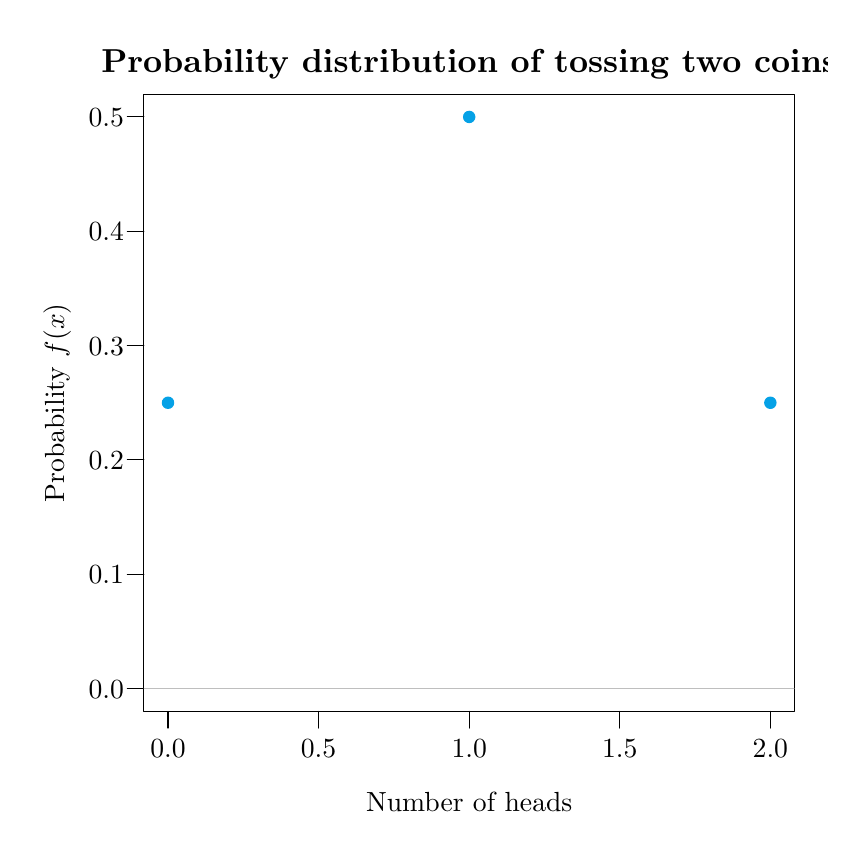
\begin{tikzpicture}[x=1pt,y=1pt]
\definecolor{fillColor}{RGB}{255,255,255}
\path[use as bounding box,fill=fillColor,fill opacity=0.00] (0,0) rectangle (289.08,289.08);
\begin{scope}
\path[clip] ( 42.00, 42.00) rectangle (277.08,265.08);
\definecolor{fillColor}{RGB}{5,161,230}

\path[fill=fillColor] ( 50.71,153.54) circle (  2.25);

\path[fill=fillColor] (159.54,256.82) circle (  2.25);

\path[fill=fillColor] (268.37,153.54) circle (  2.25);
\end{scope}
\begin{scope}
\path[clip] (  0.00,  0.00) rectangle (289.08,289.08);
\definecolor{drawColor}{RGB}{0,0,0}

\path[draw=drawColor,line width= 0.4pt,line join=round,line cap=round] ( 50.71, 42.00) -- (268.37, 42.00);

\path[draw=drawColor,line width= 0.4pt,line join=round,line cap=round] ( 50.71, 42.00) -- ( 50.71, 36.00);

\path[draw=drawColor,line width= 0.4pt,line join=round,line cap=round] (105.12, 42.00) -- (105.12, 36.00);

\path[draw=drawColor,line width= 0.4pt,line join=round,line cap=round] (159.54, 42.00) -- (159.54, 36.00);

\path[draw=drawColor,line width= 0.4pt,line join=round,line cap=round] (213.96, 42.00) -- (213.96, 36.00);

\path[draw=drawColor,line width= 0.4pt,line join=round,line cap=round] (268.37, 42.00) -- (268.37, 36.00);

\node[text=drawColor,anchor=base,inner sep=0pt, outer sep=0pt, scale=  1.00] at ( 50.71, 25.20) {0.0};

\node[text=drawColor,anchor=base,inner sep=0pt, outer sep=0pt, scale=  1.00] at (105.12, 25.20) {0.5};

\node[text=drawColor,anchor=base,inner sep=0pt, outer sep=0pt, scale=  1.00] at (159.54, 25.20) {1.0};

\node[text=drawColor,anchor=base,inner sep=0pt, outer sep=0pt, scale=  1.00] at (213.96, 25.20) {1.5};

\node[text=drawColor,anchor=base,inner sep=0pt, outer sep=0pt, scale=  1.00] at (268.37, 25.20) {2.0};

\path[draw=drawColor,line width= 0.4pt,line join=round,line cap=round] ( 42.00, 50.26) -- ( 42.00,256.82);

\path[draw=drawColor,line width= 0.4pt,line join=round,line cap=round] ( 42.00, 50.26) -- ( 36.00, 50.26);

\path[draw=drawColor,line width= 0.4pt,line join=round,line cap=round] ( 42.00, 91.57) -- ( 36.00, 91.57);

\path[draw=drawColor,line width= 0.4pt,line join=round,line cap=round] ( 42.00,132.88) -- ( 36.00,132.88);

\path[draw=drawColor,line width= 0.4pt,line join=round,line cap=round] ( 42.00,174.20) -- ( 36.00,174.20);

\path[draw=drawColor,line width= 0.4pt,line join=round,line cap=round] ( 42.00,215.51) -- ( 36.00,215.51);

\path[draw=drawColor,line width= 0.4pt,line join=round,line cap=round] ( 42.00,256.82) -- ( 36.00,256.82);

\node[text=drawColor,anchor=base east,inner sep=0pt, outer sep=0pt, scale=  1.00] at ( 34.80, 46.82) {0.0};

\node[text=drawColor,anchor=base east,inner sep=0pt, outer sep=0pt, scale=  1.00] at ( 34.80, 88.13) {0.1};

\node[text=drawColor,anchor=base east,inner sep=0pt, outer sep=0pt, scale=  1.00] at ( 34.80,129.44) {0.2};

\node[text=drawColor,anchor=base east,inner sep=0pt, outer sep=0pt, scale=  1.00] at ( 34.80,170.75) {0.3};

\node[text=drawColor,anchor=base east,inner sep=0pt, outer sep=0pt, scale=  1.00] at ( 34.80,212.06) {0.4};

\node[text=drawColor,anchor=base east,inner sep=0pt, outer sep=0pt, scale=  1.00] at ( 34.80,253.37) {0.5};

\path[draw=drawColor,line width= 0.4pt,line join=round,line cap=round] ( 42.00, 42.00) --
	(277.08, 42.00) --
	(277.08,265.08) --
	( 42.00,265.08) --
	( 42.00, 42.00);
\end{scope}
\begin{scope}
\path[clip] (  0.00,  0.00) rectangle (289.08,289.08);
\definecolor{drawColor}{RGB}{0,0,0}

\node[text=drawColor,anchor=base,inner sep=0pt, outer sep=0pt, scale=  1.20] at (159.54,272.89) {\bfseries Probability distribution of tossing two coins};

\node[text=drawColor,anchor=base,inner sep=0pt, outer sep=0pt, scale=  1.00] at (159.54,  6.00) {Number of heads};

\node[text=drawColor,rotate= 90.00,anchor=base,inner sep=0pt, outer sep=0pt, scale=  1.00] at ( 13.20,153.54) {Probability $f(x)$};
\end{scope}
\begin{scope}
\path[clip] ( 42.00, 42.00) rectangle (277.08,265.08);
\definecolor{drawColor}{RGB}{190,190,190}

\path[draw=drawColor,line width= 0.4pt,line join=round,line cap=round] ( 42.00, 50.26) -- (277.08, 50.26);
\end{scope}
\end{tikzpicture}
}}
\mode<presentation>{\resizebox{0.45\textwidth}{!}{% Created by tikzDevice version 0.10.1 on 2016-04-19 18:05:32
% !TEX encoding = UTF-8 Unicode
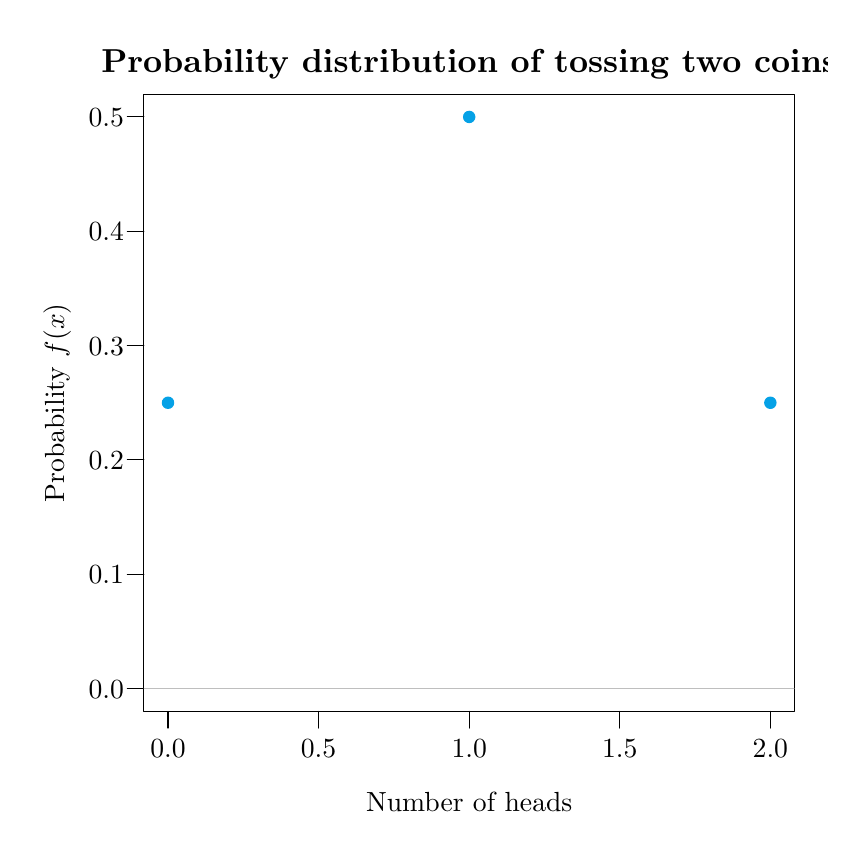
\begin{tikzpicture}[x=1pt,y=1pt]
\definecolor{fillColor}{RGB}{255,255,255}
\path[use as bounding box,fill=fillColor,fill opacity=0.00] (0,0) rectangle (289.08,289.08);
\begin{scope}
\path[clip] ( 42.00, 42.00) rectangle (277.08,265.08);
\definecolor{fillColor}{RGB}{5,161,230}

\path[fill=fillColor] ( 50.71,153.54) circle (  2.25);

\path[fill=fillColor] (159.54,256.82) circle (  2.25);

\path[fill=fillColor] (268.37,153.54) circle (  2.25);
\end{scope}
\begin{scope}
\path[clip] (  0.00,  0.00) rectangle (289.08,289.08);
\definecolor{drawColor}{RGB}{0,0,0}

\path[draw=drawColor,line width= 0.4pt,line join=round,line cap=round] ( 50.71, 42.00) -- (268.37, 42.00);

\path[draw=drawColor,line width= 0.4pt,line join=round,line cap=round] ( 50.71, 42.00) -- ( 50.71, 36.00);

\path[draw=drawColor,line width= 0.4pt,line join=round,line cap=round] (105.12, 42.00) -- (105.12, 36.00);

\path[draw=drawColor,line width= 0.4pt,line join=round,line cap=round] (159.54, 42.00) -- (159.54, 36.00);

\path[draw=drawColor,line width= 0.4pt,line join=round,line cap=round] (213.96, 42.00) -- (213.96, 36.00);

\path[draw=drawColor,line width= 0.4pt,line join=round,line cap=round] (268.37, 42.00) -- (268.37, 36.00);

\node[text=drawColor,anchor=base,inner sep=0pt, outer sep=0pt, scale=  1.00] at ( 50.71, 25.20) {0.0};

\node[text=drawColor,anchor=base,inner sep=0pt, outer sep=0pt, scale=  1.00] at (105.12, 25.20) {0.5};

\node[text=drawColor,anchor=base,inner sep=0pt, outer sep=0pt, scale=  1.00] at (159.54, 25.20) {1.0};

\node[text=drawColor,anchor=base,inner sep=0pt, outer sep=0pt, scale=  1.00] at (213.96, 25.20) {1.5};

\node[text=drawColor,anchor=base,inner sep=0pt, outer sep=0pt, scale=  1.00] at (268.37, 25.20) {2.0};

\path[draw=drawColor,line width= 0.4pt,line join=round,line cap=round] ( 42.00, 50.26) -- ( 42.00,256.82);

\path[draw=drawColor,line width= 0.4pt,line join=round,line cap=round] ( 42.00, 50.26) -- ( 36.00, 50.26);

\path[draw=drawColor,line width= 0.4pt,line join=round,line cap=round] ( 42.00, 91.57) -- ( 36.00, 91.57);

\path[draw=drawColor,line width= 0.4pt,line join=round,line cap=round] ( 42.00,132.88) -- ( 36.00,132.88);

\path[draw=drawColor,line width= 0.4pt,line join=round,line cap=round] ( 42.00,174.20) -- ( 36.00,174.20);

\path[draw=drawColor,line width= 0.4pt,line join=round,line cap=round] ( 42.00,215.51) -- ( 36.00,215.51);

\path[draw=drawColor,line width= 0.4pt,line join=round,line cap=round] ( 42.00,256.82) -- ( 36.00,256.82);

\node[text=drawColor,anchor=base east,inner sep=0pt, outer sep=0pt, scale=  1.00] at ( 34.80, 46.82) {0.0};

\node[text=drawColor,anchor=base east,inner sep=0pt, outer sep=0pt, scale=  1.00] at ( 34.80, 88.13) {0.1};

\node[text=drawColor,anchor=base east,inner sep=0pt, outer sep=0pt, scale=  1.00] at ( 34.80,129.44) {0.2};

\node[text=drawColor,anchor=base east,inner sep=0pt, outer sep=0pt, scale=  1.00] at ( 34.80,170.75) {0.3};

\node[text=drawColor,anchor=base east,inner sep=0pt, outer sep=0pt, scale=  1.00] at ( 34.80,212.06) {0.4};

\node[text=drawColor,anchor=base east,inner sep=0pt, outer sep=0pt, scale=  1.00] at ( 34.80,253.37) {0.5};

\path[draw=drawColor,line width= 0.4pt,line join=round,line cap=round] ( 42.00, 42.00) --
	(277.08, 42.00) --
	(277.08,265.08) --
	( 42.00,265.08) --
	( 42.00, 42.00);
\end{scope}
\begin{scope}
\path[clip] (  0.00,  0.00) rectangle (289.08,289.08);
\definecolor{drawColor}{RGB}{0,0,0}

\node[text=drawColor,anchor=base,inner sep=0pt, outer sep=0pt, scale=  1.20] at (159.54,272.89) {\bfseries Probability distribution of tossing two coins};

\node[text=drawColor,anchor=base,inner sep=0pt, outer sep=0pt, scale=  1.00] at (159.54,  6.00) {Number of heads};

\node[text=drawColor,rotate= 90.00,anchor=base,inner sep=0pt, outer sep=0pt, scale=  1.00] at ( 13.20,153.54) {Probability $f(x)$};
\end{scope}
\begin{scope}
\path[clip] ( 42.00, 42.00) rectangle (277.08,265.08);
\definecolor{drawColor}{RGB}{190,190,190}

\path[draw=drawColor,line width= 0.4pt,line join=round,line cap=round] ( 42.00, 50.26) -- (277.08, 50.26);
\end{scope}
\end{tikzpicture}
}}
&
\tikzsetnextfilename{discrete_random_variables/two_coins_distribution_function}
\mode<article>{\resizebox{0.45\textwidth}{!}{% Created by tikzDevice version 0.10.1 on 2016-04-19 09:52:57
% !TEX encoding = UTF-8 Unicode
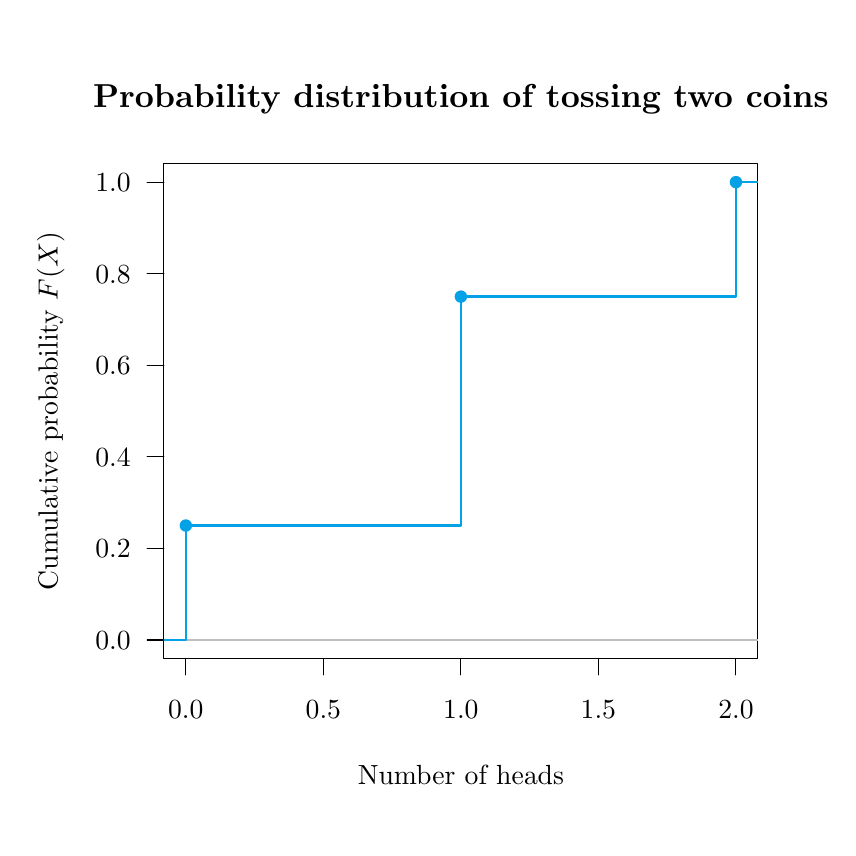
\begin{tikzpicture}[x=1pt,y=1pt]
\definecolor{fillColor}{RGB}{255,255,255}
\path[use as bounding box,fill=fillColor,fill opacity=0.00] (0,0) rectangle (289.08,289.08);
\begin{scope}
\path[clip] ( 49.20, 61.20) rectangle (263.88,239.88);
\definecolor{fillColor}{RGB}{5,161,230}

\path[fill=fillColor] ( 57.15,109.18) circle (  2.25);

\path[fill=fillColor] (156.54,191.90) circle (  2.25);

\path[fill=fillColor] (255.93,233.26) circle (  2.25);
\end{scope}
\begin{scope}
\path[clip] (  0.00,  0.00) rectangle (289.08,289.08);
\definecolor{drawColor}{RGB}{0,0,0}

\path[draw=drawColor,line width= 0.4pt,line join=round,line cap=round] ( 57.15, 61.20) -- (255.93, 61.20);

\path[draw=drawColor,line width= 0.4pt,line join=round,line cap=round] ( 57.15, 61.20) -- ( 57.15, 55.20);

\path[draw=drawColor,line width= 0.4pt,line join=round,line cap=round] (106.85, 61.20) -- (106.85, 55.20);

\path[draw=drawColor,line width= 0.4pt,line join=round,line cap=round] (156.54, 61.20) -- (156.54, 55.20);

\path[draw=drawColor,line width= 0.4pt,line join=round,line cap=round] (206.23, 61.20) -- (206.23, 55.20);

\path[draw=drawColor,line width= 0.4pt,line join=round,line cap=round] (255.93, 61.20) -- (255.93, 55.20);

\node[text=drawColor,anchor=base,inner sep=0pt, outer sep=0pt, scale=  1.00] at ( 57.15, 39.60) {0.0};

\node[text=drawColor,anchor=base,inner sep=0pt, outer sep=0pt, scale=  1.00] at (106.85, 39.60) {0.5};

\node[text=drawColor,anchor=base,inner sep=0pt, outer sep=0pt, scale=  1.00] at (156.54, 39.60) {1.0};

\node[text=drawColor,anchor=base,inner sep=0pt, outer sep=0pt, scale=  1.00] at (206.23, 39.60) {1.5};

\node[text=drawColor,anchor=base,inner sep=0pt, outer sep=0pt, scale=  1.00] at (255.93, 39.60) {2.0};

\path[draw=drawColor,line width= 0.4pt,line join=round,line cap=round] ( 49.20, 67.82) -- ( 49.20,233.26);

\path[draw=drawColor,line width= 0.4pt,line join=round,line cap=round] ( 49.20, 67.82) -- ( 43.20, 67.82);

\path[draw=drawColor,line width= 0.4pt,line join=round,line cap=round] ( 49.20,100.91) -- ( 43.20,100.91);

\path[draw=drawColor,line width= 0.4pt,line join=round,line cap=round] ( 49.20,134.00) -- ( 43.20,134.00);

\path[draw=drawColor,line width= 0.4pt,line join=round,line cap=round] ( 49.20,167.08) -- ( 43.20,167.08);

\path[draw=drawColor,line width= 0.4pt,line join=round,line cap=round] ( 49.20,200.17) -- ( 43.20,200.17);

\path[draw=drawColor,line width= 0.4pt,line join=round,line cap=round] ( 49.20,233.26) -- ( 43.20,233.26);

\node[text=drawColor,anchor=base east,inner sep=0pt, outer sep=0pt, scale=  1.00] at ( 37.20, 64.37) {0.0};

\node[text=drawColor,anchor=base east,inner sep=0pt, outer sep=0pt, scale=  1.00] at ( 37.20, 97.46) {0.2};

\node[text=drawColor,anchor=base east,inner sep=0pt, outer sep=0pt, scale=  1.00] at ( 37.20,130.55) {0.4};

\node[text=drawColor,anchor=base east,inner sep=0pt, outer sep=0pt, scale=  1.00] at ( 37.20,163.64) {0.6};

\node[text=drawColor,anchor=base east,inner sep=0pt, outer sep=0pt, scale=  1.00] at ( 37.20,196.73) {0.8};

\node[text=drawColor,anchor=base east,inner sep=0pt, outer sep=0pt, scale=  1.00] at ( 37.20,229.82) {1.0};

\path[draw=drawColor,line width= 0.4pt,line join=round,line cap=round] ( 49.20, 61.20) --
	(263.88, 61.20) --
	(263.88,239.88) --
	( 49.20,239.88) --
	( 49.20, 61.20);
\end{scope}
\begin{scope}
\path[clip] (  0.00,  0.00) rectangle (289.08,289.08);
\definecolor{drawColor}{RGB}{0,0,0}

\node[text=drawColor,anchor=base,inner sep=0pt, outer sep=0pt, scale=  1.20] at (156.54,260.29) {\bfseries Probability distribution of tossing two coins};

\node[text=drawColor,anchor=base,inner sep=0pt, outer sep=0pt, scale=  1.00] at (156.54, 15.60) {Number of heads};

\node[text=drawColor,rotate= 90.00,anchor=base,inner sep=0pt, outer sep=0pt, scale=  1.00] at ( 10.80,150.54) {Cumulative probability $F(X)$};
\end{scope}
\begin{scope}
\path[clip] ( 49.20, 61.20) rectangle (263.88,239.88);
\definecolor{drawColor}{RGB}{190,190,190}

\path[draw=drawColor,line width= 0.4pt,line join=round,line cap=round] ( 49.20, 67.82) -- (263.88, 67.82);
\definecolor{drawColor}{RGB}{5,161,230}

\path[draw=drawColor,line width= 0.8pt,line join=round,line cap=round] (  0.00, 67.82) --
	( 57.15, 67.82) --
	( 57.15,109.18) --
	(156.54,109.18) --
	(156.54,191.90) --
	(255.93,191.90) --
	(255.93,233.26) --
	(289.08,233.26);
\end{scope}
\end{tikzpicture}
}}
\mode<presentation>{\resizebox{0.45\textwidth}{!}{% Created by tikzDevice version 0.10.1 on 2016-04-19 09:52:57
% !TEX encoding = UTF-8 Unicode
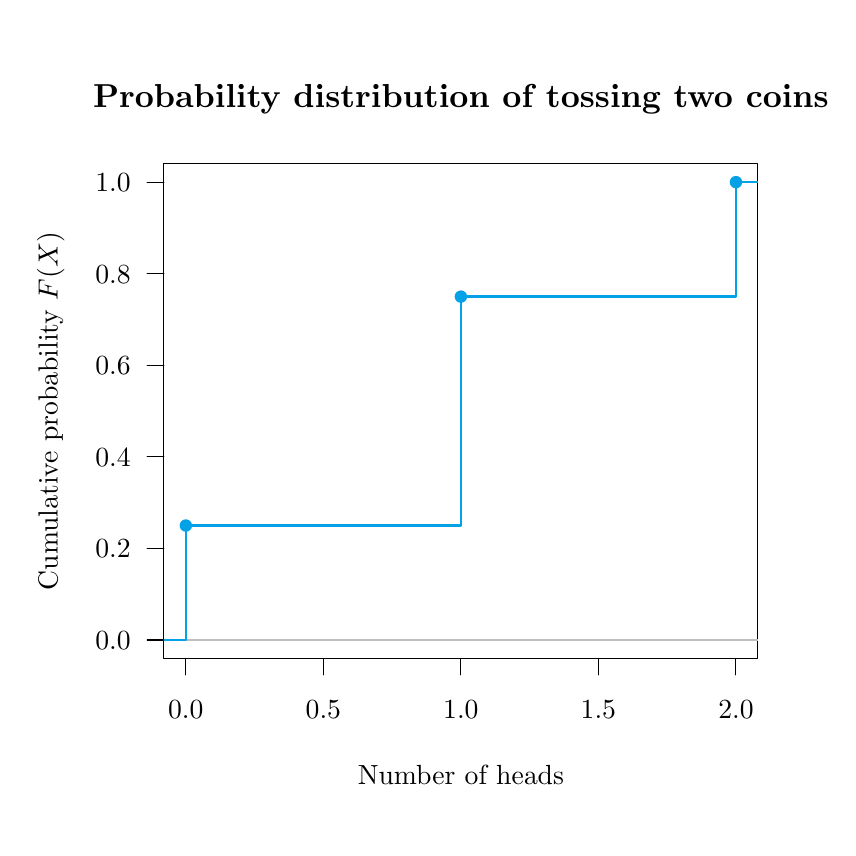
\begin{tikzpicture}[x=1pt,y=1pt]
\definecolor{fillColor}{RGB}{255,255,255}
\path[use as bounding box,fill=fillColor,fill opacity=0.00] (0,0) rectangle (289.08,289.08);
\begin{scope}
\path[clip] ( 49.20, 61.20) rectangle (263.88,239.88);
\definecolor{fillColor}{RGB}{5,161,230}

\path[fill=fillColor] ( 57.15,109.18) circle (  2.25);

\path[fill=fillColor] (156.54,191.90) circle (  2.25);

\path[fill=fillColor] (255.93,233.26) circle (  2.25);
\end{scope}
\begin{scope}
\path[clip] (  0.00,  0.00) rectangle (289.08,289.08);
\definecolor{drawColor}{RGB}{0,0,0}

\path[draw=drawColor,line width= 0.4pt,line join=round,line cap=round] ( 57.15, 61.20) -- (255.93, 61.20);

\path[draw=drawColor,line width= 0.4pt,line join=round,line cap=round] ( 57.15, 61.20) -- ( 57.15, 55.20);

\path[draw=drawColor,line width= 0.4pt,line join=round,line cap=round] (106.85, 61.20) -- (106.85, 55.20);

\path[draw=drawColor,line width= 0.4pt,line join=round,line cap=round] (156.54, 61.20) -- (156.54, 55.20);

\path[draw=drawColor,line width= 0.4pt,line join=round,line cap=round] (206.23, 61.20) -- (206.23, 55.20);

\path[draw=drawColor,line width= 0.4pt,line join=round,line cap=round] (255.93, 61.20) -- (255.93, 55.20);

\node[text=drawColor,anchor=base,inner sep=0pt, outer sep=0pt, scale=  1.00] at ( 57.15, 39.60) {0.0};

\node[text=drawColor,anchor=base,inner sep=0pt, outer sep=0pt, scale=  1.00] at (106.85, 39.60) {0.5};

\node[text=drawColor,anchor=base,inner sep=0pt, outer sep=0pt, scale=  1.00] at (156.54, 39.60) {1.0};

\node[text=drawColor,anchor=base,inner sep=0pt, outer sep=0pt, scale=  1.00] at (206.23, 39.60) {1.5};

\node[text=drawColor,anchor=base,inner sep=0pt, outer sep=0pt, scale=  1.00] at (255.93, 39.60) {2.0};

\path[draw=drawColor,line width= 0.4pt,line join=round,line cap=round] ( 49.20, 67.82) -- ( 49.20,233.26);

\path[draw=drawColor,line width= 0.4pt,line join=round,line cap=round] ( 49.20, 67.82) -- ( 43.20, 67.82);

\path[draw=drawColor,line width= 0.4pt,line join=round,line cap=round] ( 49.20,100.91) -- ( 43.20,100.91);

\path[draw=drawColor,line width= 0.4pt,line join=round,line cap=round] ( 49.20,134.00) -- ( 43.20,134.00);

\path[draw=drawColor,line width= 0.4pt,line join=round,line cap=round] ( 49.20,167.08) -- ( 43.20,167.08);

\path[draw=drawColor,line width= 0.4pt,line join=round,line cap=round] ( 49.20,200.17) -- ( 43.20,200.17);

\path[draw=drawColor,line width= 0.4pt,line join=round,line cap=round] ( 49.20,233.26) -- ( 43.20,233.26);

\node[text=drawColor,anchor=base east,inner sep=0pt, outer sep=0pt, scale=  1.00] at ( 37.20, 64.37) {0.0};

\node[text=drawColor,anchor=base east,inner sep=0pt, outer sep=0pt, scale=  1.00] at ( 37.20, 97.46) {0.2};

\node[text=drawColor,anchor=base east,inner sep=0pt, outer sep=0pt, scale=  1.00] at ( 37.20,130.55) {0.4};

\node[text=drawColor,anchor=base east,inner sep=0pt, outer sep=0pt, scale=  1.00] at ( 37.20,163.64) {0.6};

\node[text=drawColor,anchor=base east,inner sep=0pt, outer sep=0pt, scale=  1.00] at ( 37.20,196.73) {0.8};

\node[text=drawColor,anchor=base east,inner sep=0pt, outer sep=0pt, scale=  1.00] at ( 37.20,229.82) {1.0};

\path[draw=drawColor,line width= 0.4pt,line join=round,line cap=round] ( 49.20, 61.20) --
	(263.88, 61.20) --
	(263.88,239.88) --
	( 49.20,239.88) --
	( 49.20, 61.20);
\end{scope}
\begin{scope}
\path[clip] (  0.00,  0.00) rectangle (289.08,289.08);
\definecolor{drawColor}{RGB}{0,0,0}

\node[text=drawColor,anchor=base,inner sep=0pt, outer sep=0pt, scale=  1.20] at (156.54,260.29) {\bfseries Probability distribution of tossing two coins};

\node[text=drawColor,anchor=base,inner sep=0pt, outer sep=0pt, scale=  1.00] at (156.54, 15.60) {Number of heads};

\node[text=drawColor,rotate= 90.00,anchor=base,inner sep=0pt, outer sep=0pt, scale=  1.00] at ( 10.80,150.54) {Cumulative probability $F(X)$};
\end{scope}
\begin{scope}
\path[clip] ( 49.20, 61.20) rectangle (263.88,239.88);
\definecolor{drawColor}{RGB}{190,190,190}

\path[draw=drawColor,line width= 0.4pt,line join=round,line cap=round] ( 49.20, 67.82) -- (263.88, 67.82);
\definecolor{drawColor}{RGB}{5,161,230}

\path[draw=drawColor,line width= 0.8pt,line join=round,line cap=round] (  0.00, 67.82) --
	( 57.15, 67.82) --
	( 57.15,109.18) --
	(156.54,109.18) --
	(156.54,191.90) --
	(255.93,191.90) --
	(255.93,233.26) --
	(289.08,233.26);
\end{scope}
\end{tikzpicture}
}}
\end{tabular}
\end{center} 
\end{frame}


%---------------------------------------------------------------------slide----
\begin{frame}
\frametitle{Population statistics}
The same way we use sample statistics to describe the sample frequency distribution of a variable, we use
population statistics to describe the probability distribution of a random variable in the whole population.

The population statistics definition is analogous to the sample statistics definition, but using probabilities
instead of relative frequencies. 

The most important are \footnote{To distinguish population statistics from sample statistics we use Greek letters}:
\begin{itemize}
\item \structure{Mean}:
\[
\mu = E(X) = \sum_{i=1}^n x_i f(x_i)
\]
\item \structure{Variance}:
\[
\sigma^2 = Var(X) = \sum_{i=1}^n x_i^2 f(x_i) -\mu^2
\]
\item \structure{Standard deviation}:
\[
\sigma = +\sqrt{\sigma^2}
\]
\end{itemize}
\end{frame}


%---------------------------------------------------------------------slide----
\begin{frame}
\frametitle{Population statistics}
\framesubtitle{Example of tossing two coins}
In the random experiment of tossing two coins the probability distribution is  
\[
\begin{array}{|c|ccc|}
\hline
X & 0 & 1 & 2\\ \hline
f(x) & 0.25 & 0.5 & 0.25\\
\hline
F(x) & 0.25 & 0.75 & 1 \\
\hline
\end{array}
\]

The main population statistics are 
\begin{align*}
\mu &= \sum_{i=1}^n x_i f(x_i) = 0\cdot 0.25 + 1\cdot 0.5 + 2\cdot 0.25 = 1 \mbox{ heads},\\
\sigma^2 &= \sum_{i=1}^n x_i^2 f(x_i) -\mu^2 = (0^0\cdot 0.25 + 1^2\cdot 0.5 + 2^2\cdot 0.25) - 1^2 = 0.5 \mbox{
heads}^2,\\
\sigma &= +\sqrt{0.5} = 0.71 \mbox{ heads}.
\end{align*}
\end{frame}


%---------------------------------------------------------------------slide----
\begin{frame}
\frametitle{Discrete probability distribution models}
According to the type of experiment where the random variable is measured, there are different probability distributions
models. 
The most common are

\begin{itemize}
\item Discrete uniform
\item Binomial
\item Poisson 
\end{itemize}
\end{frame}


\subsection{Discrete uniform distribution}

% ---------------------------------------------------------------------slide----
\begin{frame}
\frametitle{Discrete uniform probability distribution model $U(a,b)$}
When all the values of a random variable $X$ have equal probability, the probability distribution of $X$ is uniform.

\begin{definition}[Discrete uniform distribution $U(a,b)$]
A discrete random variable $X$ follows a \emph{discrete uniform distribution model} with parameters $a$ and $b$, noted 
$X\sim U(a,b)$, if its range is $\mbox{Ran}(X) = \{a, a+1, \ldots,b\}$ and its probability function is
\[f(x)=\frac{1}{b-a+1}.\]
\end{definition}

Observe that $a$ and $b$ are the minimum and the maximum of the range respectively. 

The mean and the variance are
\[
\mu = \sum_{i=0}^{b-a}\frac{a+i}{b-a+1}=\frac{a+b}{2} \qquad \sigma^2 =\sum_{i=0}^{b-a}\frac{(a+i-\mu)^2}{b-a+1}=
\frac{(b-a+1)^2-1}{12}
\]
\end{frame}


%---------------------------------------------------------------------slide----
\begin{frame}
\frametitle{Discrete uniform probability distribution model $U(a,b)$}
\framesubtitle{Example of rolling a dice}
The variable that measures the outcome of rolling a dice follows a discrete uniform distribution model $U(1,6)$.
\begin{center}
\tikzsetnextfilename{discrete_random_variables/discrete_uniform_probability_function}
\mode<article>{\resizebox{0.5\textwidth}{!}{% Created by tikzDevice version 0.10.1 on 2016-04-19 09:52:58
% !TEX encoding = UTF-8 Unicode
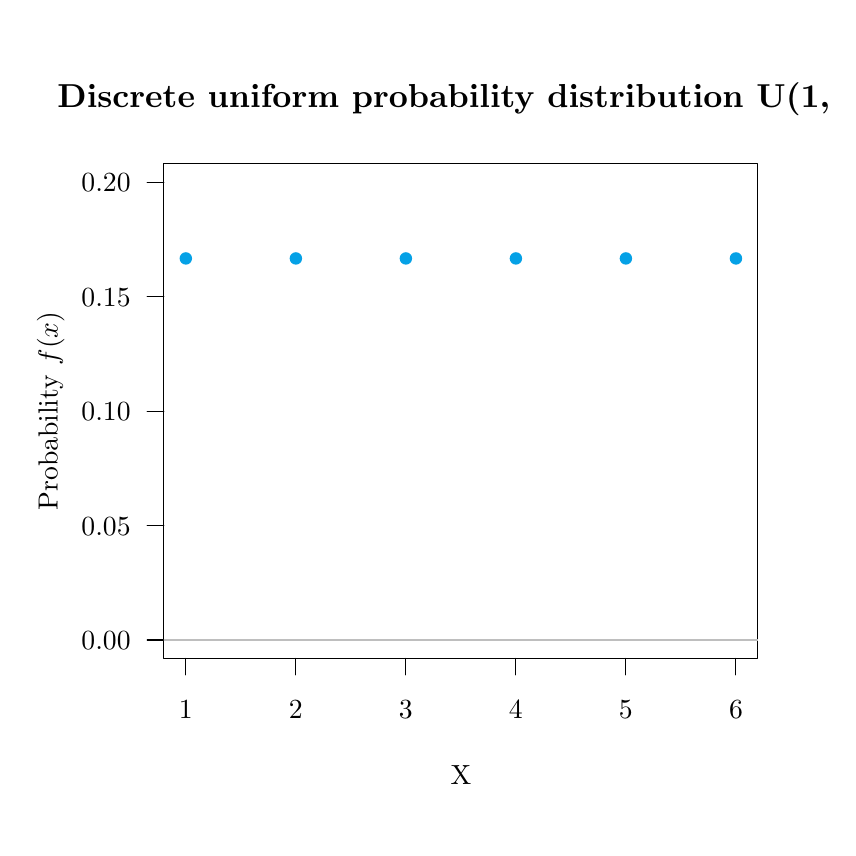
\begin{tikzpicture}[x=1pt,y=1pt]
\definecolor{fillColor}{RGB}{255,255,255}
\path[use as bounding box,fill=fillColor,fill opacity=0.00] (0,0) rectangle (289.08,289.08);
\begin{scope}
\path[clip] ( 49.20, 61.20) rectangle (263.88,239.88);
\definecolor{fillColor}{RGB}{5,161,230}

\path[fill=fillColor] ( 57.15,205.69) circle (  2.25);

\path[fill=fillColor] ( 96.91,205.69) circle (  2.25);

\path[fill=fillColor] (136.66,205.69) circle (  2.25);

\path[fill=fillColor] (176.42,205.69) circle (  2.25);

\path[fill=fillColor] (216.17,205.69) circle (  2.25);

\path[fill=fillColor] (255.93,205.69) circle (  2.25);
\end{scope}
\begin{scope}
\path[clip] (  0.00,  0.00) rectangle (289.08,289.08);
\definecolor{drawColor}{RGB}{0,0,0}

\path[draw=drawColor,line width= 0.4pt,line join=round,line cap=round] ( 57.15, 61.20) -- (255.93, 61.20);

\path[draw=drawColor,line width= 0.4pt,line join=round,line cap=round] ( 57.15, 61.20) -- ( 57.15, 55.20);

\path[draw=drawColor,line width= 0.4pt,line join=round,line cap=round] ( 96.91, 61.20) -- ( 96.91, 55.20);

\path[draw=drawColor,line width= 0.4pt,line join=round,line cap=round] (136.66, 61.20) -- (136.66, 55.20);

\path[draw=drawColor,line width= 0.4pt,line join=round,line cap=round] (176.42, 61.20) -- (176.42, 55.20);

\path[draw=drawColor,line width= 0.4pt,line join=round,line cap=round] (216.17, 61.20) -- (216.17, 55.20);

\path[draw=drawColor,line width= 0.4pt,line join=round,line cap=round] (255.93, 61.20) -- (255.93, 55.20);

\node[text=drawColor,anchor=base,inner sep=0pt, outer sep=0pt, scale=  1.00] at ( 57.15, 39.60) {1};

\node[text=drawColor,anchor=base,inner sep=0pt, outer sep=0pt, scale=  1.00] at ( 96.91, 39.60) {2};

\node[text=drawColor,anchor=base,inner sep=0pt, outer sep=0pt, scale=  1.00] at (136.66, 39.60) {3};

\node[text=drawColor,anchor=base,inner sep=0pt, outer sep=0pt, scale=  1.00] at (176.42, 39.60) {4};

\node[text=drawColor,anchor=base,inner sep=0pt, outer sep=0pt, scale=  1.00] at (216.17, 39.60) {5};

\node[text=drawColor,anchor=base,inner sep=0pt, outer sep=0pt, scale=  1.00] at (255.93, 39.60) {6};

\path[draw=drawColor,line width= 0.4pt,line join=round,line cap=round] ( 49.20, 67.82) -- ( 49.20,233.26);

\path[draw=drawColor,line width= 0.4pt,line join=round,line cap=round] ( 49.20, 67.82) -- ( 43.20, 67.82);

\path[draw=drawColor,line width= 0.4pt,line join=round,line cap=round] ( 49.20,109.18) -- ( 43.20,109.18);

\path[draw=drawColor,line width= 0.4pt,line join=round,line cap=round] ( 49.20,150.54) -- ( 43.20,150.54);

\path[draw=drawColor,line width= 0.4pt,line join=round,line cap=round] ( 49.20,191.90) -- ( 43.20,191.90);

\path[draw=drawColor,line width= 0.4pt,line join=round,line cap=round] ( 49.20,233.26) -- ( 43.20,233.26);

\node[text=drawColor,anchor=base east,inner sep=0pt, outer sep=0pt, scale=  1.00] at ( 37.20, 64.37) {0.00};

\node[text=drawColor,anchor=base east,inner sep=0pt, outer sep=0pt, scale=  1.00] at ( 37.20,105.73) {0.05};

\node[text=drawColor,anchor=base east,inner sep=0pt, outer sep=0pt, scale=  1.00] at ( 37.20,147.10) {0.10};

\node[text=drawColor,anchor=base east,inner sep=0pt, outer sep=0pt, scale=  1.00] at ( 37.20,188.46) {0.15};

\node[text=drawColor,anchor=base east,inner sep=0pt, outer sep=0pt, scale=  1.00] at ( 37.20,229.82) {0.20};

\path[draw=drawColor,line width= 0.4pt,line join=round,line cap=round] ( 49.20, 61.20) --
	(263.88, 61.20) --
	(263.88,239.88) --
	( 49.20,239.88) --
	( 49.20, 61.20);
\end{scope}
\begin{scope}
\path[clip] (  0.00,  0.00) rectangle (289.08,289.08);
\definecolor{drawColor}{RGB}{0,0,0}

\node[text=drawColor,anchor=base,inner sep=0pt, outer sep=0pt, scale=  1.20] at (156.54,260.29) {\bfseries Discrete uniform probability distribution U(1,6)};

\node[text=drawColor,anchor=base,inner sep=0pt, outer sep=0pt, scale=  1.00] at (156.54, 15.60) {X};

\node[text=drawColor,rotate= 90.00,anchor=base,inner sep=0pt, outer sep=0pt, scale=  1.00] at ( 10.80,150.54) {Probability $f(x)$};
\end{scope}
\begin{scope}
\path[clip] ( 49.20, 61.20) rectangle (263.88,239.88);
\definecolor{drawColor}{RGB}{190,190,190}

\path[draw=drawColor,line width= 0.4pt,line join=round,line cap=round] ( 49.20, 67.82) -- (263.88, 67.82);
\end{scope}
\end{tikzpicture}
}}
\mode<presentation>{\resizebox{0.55\textwidth}{!}{% Created by tikzDevice version 0.10.1 on 2016-04-19 09:52:58
% !TEX encoding = UTF-8 Unicode
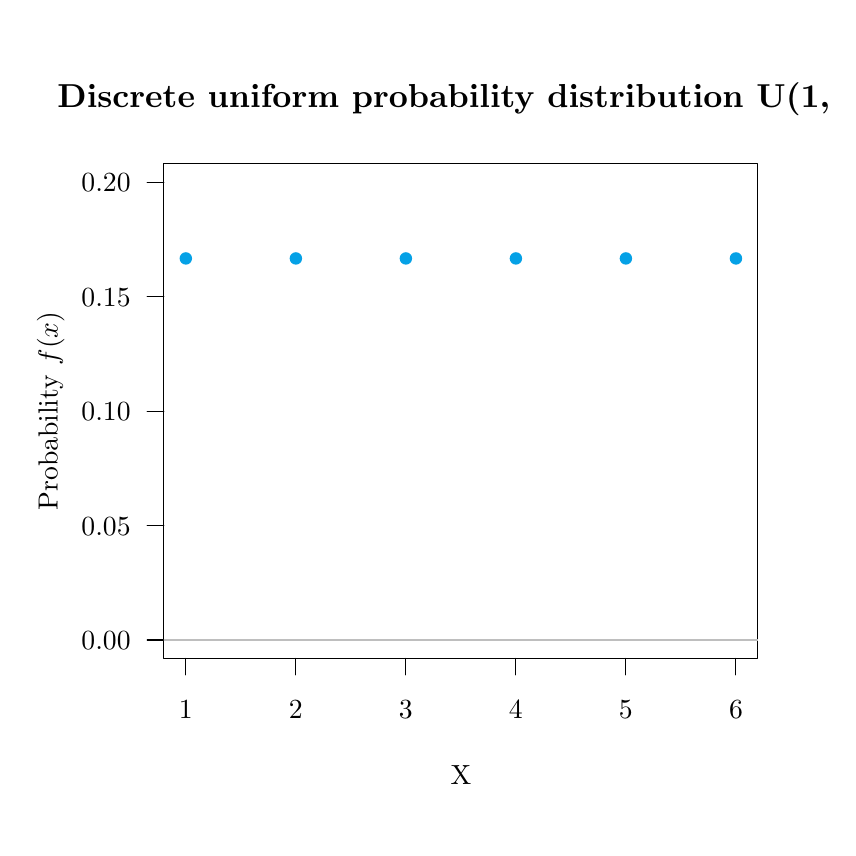
\begin{tikzpicture}[x=1pt,y=1pt]
\definecolor{fillColor}{RGB}{255,255,255}
\path[use as bounding box,fill=fillColor,fill opacity=0.00] (0,0) rectangle (289.08,289.08);
\begin{scope}
\path[clip] ( 49.20, 61.20) rectangle (263.88,239.88);
\definecolor{fillColor}{RGB}{5,161,230}

\path[fill=fillColor] ( 57.15,205.69) circle (  2.25);

\path[fill=fillColor] ( 96.91,205.69) circle (  2.25);

\path[fill=fillColor] (136.66,205.69) circle (  2.25);

\path[fill=fillColor] (176.42,205.69) circle (  2.25);

\path[fill=fillColor] (216.17,205.69) circle (  2.25);

\path[fill=fillColor] (255.93,205.69) circle (  2.25);
\end{scope}
\begin{scope}
\path[clip] (  0.00,  0.00) rectangle (289.08,289.08);
\definecolor{drawColor}{RGB}{0,0,0}

\path[draw=drawColor,line width= 0.4pt,line join=round,line cap=round] ( 57.15, 61.20) -- (255.93, 61.20);

\path[draw=drawColor,line width= 0.4pt,line join=round,line cap=round] ( 57.15, 61.20) -- ( 57.15, 55.20);

\path[draw=drawColor,line width= 0.4pt,line join=round,line cap=round] ( 96.91, 61.20) -- ( 96.91, 55.20);

\path[draw=drawColor,line width= 0.4pt,line join=round,line cap=round] (136.66, 61.20) -- (136.66, 55.20);

\path[draw=drawColor,line width= 0.4pt,line join=round,line cap=round] (176.42, 61.20) -- (176.42, 55.20);

\path[draw=drawColor,line width= 0.4pt,line join=round,line cap=round] (216.17, 61.20) -- (216.17, 55.20);

\path[draw=drawColor,line width= 0.4pt,line join=round,line cap=round] (255.93, 61.20) -- (255.93, 55.20);

\node[text=drawColor,anchor=base,inner sep=0pt, outer sep=0pt, scale=  1.00] at ( 57.15, 39.60) {1};

\node[text=drawColor,anchor=base,inner sep=0pt, outer sep=0pt, scale=  1.00] at ( 96.91, 39.60) {2};

\node[text=drawColor,anchor=base,inner sep=0pt, outer sep=0pt, scale=  1.00] at (136.66, 39.60) {3};

\node[text=drawColor,anchor=base,inner sep=0pt, outer sep=0pt, scale=  1.00] at (176.42, 39.60) {4};

\node[text=drawColor,anchor=base,inner sep=0pt, outer sep=0pt, scale=  1.00] at (216.17, 39.60) {5};

\node[text=drawColor,anchor=base,inner sep=0pt, outer sep=0pt, scale=  1.00] at (255.93, 39.60) {6};

\path[draw=drawColor,line width= 0.4pt,line join=round,line cap=round] ( 49.20, 67.82) -- ( 49.20,233.26);

\path[draw=drawColor,line width= 0.4pt,line join=round,line cap=round] ( 49.20, 67.82) -- ( 43.20, 67.82);

\path[draw=drawColor,line width= 0.4pt,line join=round,line cap=round] ( 49.20,109.18) -- ( 43.20,109.18);

\path[draw=drawColor,line width= 0.4pt,line join=round,line cap=round] ( 49.20,150.54) -- ( 43.20,150.54);

\path[draw=drawColor,line width= 0.4pt,line join=round,line cap=round] ( 49.20,191.90) -- ( 43.20,191.90);

\path[draw=drawColor,line width= 0.4pt,line join=round,line cap=round] ( 49.20,233.26) -- ( 43.20,233.26);

\node[text=drawColor,anchor=base east,inner sep=0pt, outer sep=0pt, scale=  1.00] at ( 37.20, 64.37) {0.00};

\node[text=drawColor,anchor=base east,inner sep=0pt, outer sep=0pt, scale=  1.00] at ( 37.20,105.73) {0.05};

\node[text=drawColor,anchor=base east,inner sep=0pt, outer sep=0pt, scale=  1.00] at ( 37.20,147.10) {0.10};

\node[text=drawColor,anchor=base east,inner sep=0pt, outer sep=0pt, scale=  1.00] at ( 37.20,188.46) {0.15};

\node[text=drawColor,anchor=base east,inner sep=0pt, outer sep=0pt, scale=  1.00] at ( 37.20,229.82) {0.20};

\path[draw=drawColor,line width= 0.4pt,line join=round,line cap=round] ( 49.20, 61.20) --
	(263.88, 61.20) --
	(263.88,239.88) --
	( 49.20,239.88) --
	( 49.20, 61.20);
\end{scope}
\begin{scope}
\path[clip] (  0.00,  0.00) rectangle (289.08,289.08);
\definecolor{drawColor}{RGB}{0,0,0}

\node[text=drawColor,anchor=base,inner sep=0pt, outer sep=0pt, scale=  1.20] at (156.54,260.29) {\bfseries Discrete uniform probability distribution U(1,6)};

\node[text=drawColor,anchor=base,inner sep=0pt, outer sep=0pt, scale=  1.00] at (156.54, 15.60) {X};

\node[text=drawColor,rotate= 90.00,anchor=base,inner sep=0pt, outer sep=0pt, scale=  1.00] at ( 10.80,150.54) {Probability $f(x)$};
\end{scope}
\begin{scope}
\path[clip] ( 49.20, 61.20) rectangle (263.88,239.88);
\definecolor{drawColor}{RGB}{190,190,190}

\path[draw=drawColor,line width= 0.4pt,line join=round,line cap=round] ( 49.20, 67.82) -- (263.88, 67.82);
\end{scope}
\end{tikzpicture}
}}
\end{center}
\end{frame}


\subsection{Binomial distribution}

%---------------------------------------------------------------------slide----
\begin{frame}
\frametitle{Binomial distribution}
Usually the binomial distribution correspond to a variable measured in a random experiment with the following features:
\begin{itemize}
\item The experiment consist in a sequence of $n$ repetitions of the same trial.
\item Each trial is repeated in identical conditions and produces two possible outcomes known as \emph{Success} or
\emph{Failure}.
\item The trials are independent among them.
\item The probability of Success is the same in all the trials and is $P(\mbox{Success})=p$.
\end{itemize}

Under these conditions, the discrete random variable $X$ that measures the number of successes in the $n$ trials follows
a \emph{binomial distribution model} with parameters $n$ and $p$.
\end{frame}


%---------------------------------------------------------------------slide----
\begin{frame}
\frametitle{Binomial distribution model $B(n,p)$}
\begin{definition}[Binomial distribution $(B(n,p)$]
A discrete random variable $X$ follows a \emph{binomial distribution model} with parameters $n$ and $p$, noted 
$X\sim B(n,p)$, if its range is $\mbox{Ran}(X) = \{0,1,\ldots,n\}$ and its probability function is
\[
f(x) = \binom{n}{x}p^x(1-p)^{n-x} = \frac{n!}{x!(n-x)!}p^x(1-p)^{n-x}.
\]
\end{definition}

Observe that $n$ is known as the number of repetitions of a trial and $p$ is known as the probability of Success in
every repetition. 

The mean and the variance are
\[
\mu = n\cdot p \qquad \sigma^2 = n\cdot p\cdot (1-p).
\]
\end{frame}


%---------------------------------------------------------------------slide----
\begin{frame}
\frametitle{Binomial distribution model $B(n,p)$}
\framesubtitle{Example of tossing 10 coins}
The variable that measures the number of heads after tossing 10 coins follows a binomial distribution model $B(10,0.5)$.
\begin{center}
\tikzsetnextfilename{discrete_random_variables/binomial_probability_function}
\mode<article>{\resizebox{0.5\textwidth}{!}{% Created by tikzDevice version 0.10.1 on 2016-04-19 09:54:30
% !TEX encoding = UTF-8 Unicode
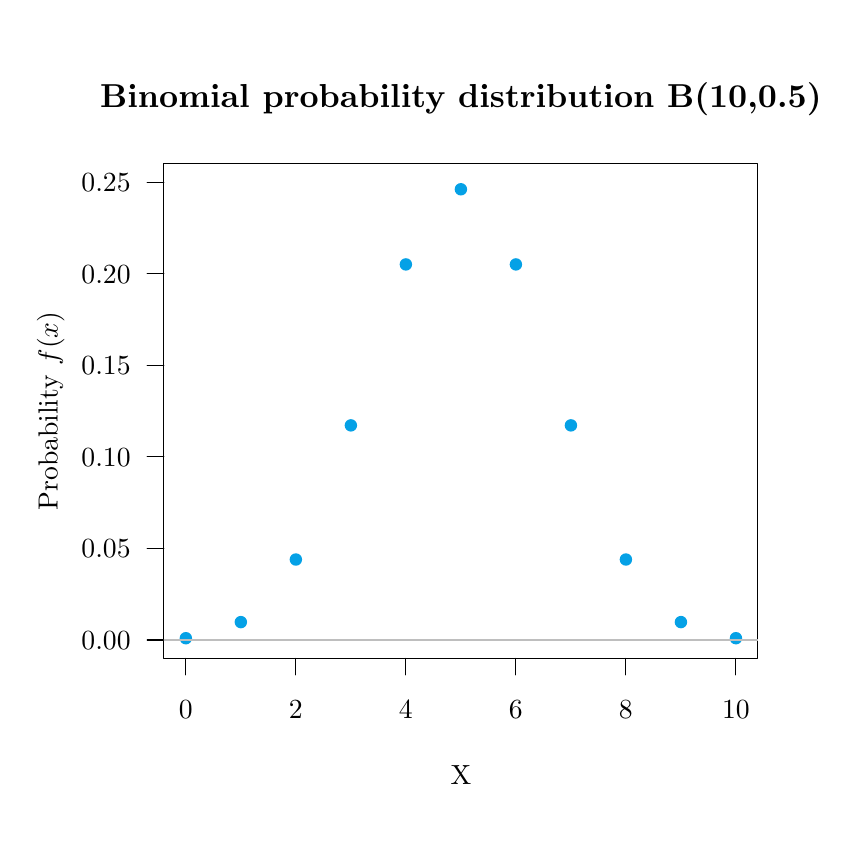
\begin{tikzpicture}[x=1pt,y=1pt]
\definecolor{fillColor}{RGB}{255,255,255}
\path[use as bounding box,fill=fillColor,fill opacity=0.00] (0,0) rectangle (289.08,289.08);
\begin{scope}
\path[clip] ( 49.20, 61.20) rectangle (263.88,239.88);
\definecolor{fillColor}{RGB}{5,161,230}

\path[fill=fillColor] ( 57.15, 68.46) circle (  2.25);

\path[fill=fillColor] ( 77.03, 74.28) circle (  2.25);

\path[fill=fillColor] ( 96.91, 96.90) circle (  2.25);

\path[fill=fillColor] (116.78,145.37) circle (  2.25);

\path[fill=fillColor] (136.66,203.53) circle (  2.25);

\path[fill=fillColor] (156.54,230.68) circle (  2.25);

\path[fill=fillColor] (176.42,203.53) circle (  2.25);

\path[fill=fillColor] (196.30,145.37) circle (  2.25);

\path[fill=fillColor] (216.17, 96.90) circle (  2.25);

\path[fill=fillColor] (236.05, 74.28) circle (  2.25);

\path[fill=fillColor] (255.93, 68.46) circle (  2.25);
\end{scope}
\begin{scope}
\path[clip] (  0.00,  0.00) rectangle (289.08,289.08);
\definecolor{drawColor}{RGB}{0,0,0}

\path[draw=drawColor,line width= 0.4pt,line join=round,line cap=round] ( 57.15, 61.20) -- (255.93, 61.20);

\path[draw=drawColor,line width= 0.4pt,line join=round,line cap=round] ( 57.15, 61.20) -- ( 57.15, 55.20);

\path[draw=drawColor,line width= 0.4pt,line join=round,line cap=round] ( 96.91, 61.20) -- ( 96.91, 55.20);

\path[draw=drawColor,line width= 0.4pt,line join=round,line cap=round] (136.66, 61.20) -- (136.66, 55.20);

\path[draw=drawColor,line width= 0.4pt,line join=round,line cap=round] (176.42, 61.20) -- (176.42, 55.20);

\path[draw=drawColor,line width= 0.4pt,line join=round,line cap=round] (216.17, 61.20) -- (216.17, 55.20);

\path[draw=drawColor,line width= 0.4pt,line join=round,line cap=round] (255.93, 61.20) -- (255.93, 55.20);

\node[text=drawColor,anchor=base,inner sep=0pt, outer sep=0pt, scale=  1.00] at ( 57.15, 39.60) {0};

\node[text=drawColor,anchor=base,inner sep=0pt, outer sep=0pt, scale=  1.00] at ( 96.91, 39.60) {2};

\node[text=drawColor,anchor=base,inner sep=0pt, outer sep=0pt, scale=  1.00] at (136.66, 39.60) {4};

\node[text=drawColor,anchor=base,inner sep=0pt, outer sep=0pt, scale=  1.00] at (176.42, 39.60) {6};

\node[text=drawColor,anchor=base,inner sep=0pt, outer sep=0pt, scale=  1.00] at (216.17, 39.60) {8};

\node[text=drawColor,anchor=base,inner sep=0pt, outer sep=0pt, scale=  1.00] at (255.93, 39.60) {10};

\path[draw=drawColor,line width= 0.4pt,line join=round,line cap=round] ( 49.20, 67.82) -- ( 49.20,233.26);

\path[draw=drawColor,line width= 0.4pt,line join=round,line cap=round] ( 49.20, 67.82) -- ( 43.20, 67.82);

\path[draw=drawColor,line width= 0.4pt,line join=round,line cap=round] ( 49.20,100.91) -- ( 43.20,100.91);

\path[draw=drawColor,line width= 0.4pt,line join=round,line cap=round] ( 49.20,134.00) -- ( 43.20,134.00);

\path[draw=drawColor,line width= 0.4pt,line join=round,line cap=round] ( 49.20,167.08) -- ( 43.20,167.08);

\path[draw=drawColor,line width= 0.4pt,line join=round,line cap=round] ( 49.20,200.17) -- ( 43.20,200.17);

\path[draw=drawColor,line width= 0.4pt,line join=round,line cap=round] ( 49.20,233.26) -- ( 43.20,233.26);

\node[text=drawColor,anchor=base east,inner sep=0pt, outer sep=0pt, scale=  1.00] at ( 37.20, 64.37) {0.00};

\node[text=drawColor,anchor=base east,inner sep=0pt, outer sep=0pt, scale=  1.00] at ( 37.20, 97.46) {0.05};

\node[text=drawColor,anchor=base east,inner sep=0pt, outer sep=0pt, scale=  1.00] at ( 37.20,130.55) {0.10};

\node[text=drawColor,anchor=base east,inner sep=0pt, outer sep=0pt, scale=  1.00] at ( 37.20,163.64) {0.15};

\node[text=drawColor,anchor=base east,inner sep=0pt, outer sep=0pt, scale=  1.00] at ( 37.20,196.73) {0.20};

\node[text=drawColor,anchor=base east,inner sep=0pt, outer sep=0pt, scale=  1.00] at ( 37.20,229.82) {0.25};

\path[draw=drawColor,line width= 0.4pt,line join=round,line cap=round] ( 49.20, 61.20) --
	(263.88, 61.20) --
	(263.88,239.88) --
	( 49.20,239.88) --
	( 49.20, 61.20);
\end{scope}
\begin{scope}
\path[clip] (  0.00,  0.00) rectangle (289.08,289.08);
\definecolor{drawColor}{RGB}{0,0,0}

\node[text=drawColor,anchor=base,inner sep=0pt, outer sep=0pt, scale=  1.20] at (156.54,260.29) {\bfseries Binomial probability distribution B(10,0.5)};

\node[text=drawColor,anchor=base,inner sep=0pt, outer sep=0pt, scale=  1.00] at (156.54, 15.60) {X};

\node[text=drawColor,rotate= 90.00,anchor=base,inner sep=0pt, outer sep=0pt, scale=  1.00] at ( 10.80,150.54) {Probability $f(x)$};
\end{scope}
\begin{scope}
\path[clip] ( 49.20, 61.20) rectangle (263.88,239.88);
\definecolor{drawColor}{RGB}{190,190,190}

\path[draw=drawColor,line width= 0.4pt,line join=round,line cap=round] ( 49.20, 67.82) -- (263.88, 67.82);
\end{scope}
\end{tikzpicture}
}}
\mode<presentation>{\resizebox{0.55\textwidth}{!}{% Created by tikzDevice version 0.10.1 on 2016-04-19 09:54:30
% !TEX encoding = UTF-8 Unicode
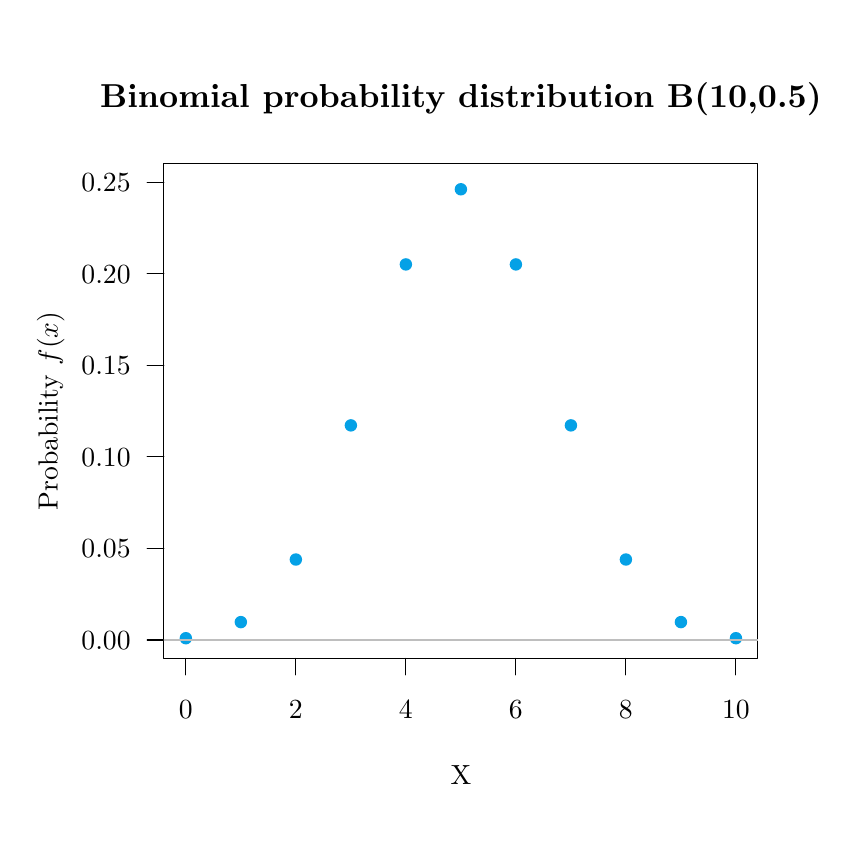
\begin{tikzpicture}[x=1pt,y=1pt]
\definecolor{fillColor}{RGB}{255,255,255}
\path[use as bounding box,fill=fillColor,fill opacity=0.00] (0,0) rectangle (289.08,289.08);
\begin{scope}
\path[clip] ( 49.20, 61.20) rectangle (263.88,239.88);
\definecolor{fillColor}{RGB}{5,161,230}

\path[fill=fillColor] ( 57.15, 68.46) circle (  2.25);

\path[fill=fillColor] ( 77.03, 74.28) circle (  2.25);

\path[fill=fillColor] ( 96.91, 96.90) circle (  2.25);

\path[fill=fillColor] (116.78,145.37) circle (  2.25);

\path[fill=fillColor] (136.66,203.53) circle (  2.25);

\path[fill=fillColor] (156.54,230.68) circle (  2.25);

\path[fill=fillColor] (176.42,203.53) circle (  2.25);

\path[fill=fillColor] (196.30,145.37) circle (  2.25);

\path[fill=fillColor] (216.17, 96.90) circle (  2.25);

\path[fill=fillColor] (236.05, 74.28) circle (  2.25);

\path[fill=fillColor] (255.93, 68.46) circle (  2.25);
\end{scope}
\begin{scope}
\path[clip] (  0.00,  0.00) rectangle (289.08,289.08);
\definecolor{drawColor}{RGB}{0,0,0}

\path[draw=drawColor,line width= 0.4pt,line join=round,line cap=round] ( 57.15, 61.20) -- (255.93, 61.20);

\path[draw=drawColor,line width= 0.4pt,line join=round,line cap=round] ( 57.15, 61.20) -- ( 57.15, 55.20);

\path[draw=drawColor,line width= 0.4pt,line join=round,line cap=round] ( 96.91, 61.20) -- ( 96.91, 55.20);

\path[draw=drawColor,line width= 0.4pt,line join=round,line cap=round] (136.66, 61.20) -- (136.66, 55.20);

\path[draw=drawColor,line width= 0.4pt,line join=round,line cap=round] (176.42, 61.20) -- (176.42, 55.20);

\path[draw=drawColor,line width= 0.4pt,line join=round,line cap=round] (216.17, 61.20) -- (216.17, 55.20);

\path[draw=drawColor,line width= 0.4pt,line join=round,line cap=round] (255.93, 61.20) -- (255.93, 55.20);

\node[text=drawColor,anchor=base,inner sep=0pt, outer sep=0pt, scale=  1.00] at ( 57.15, 39.60) {0};

\node[text=drawColor,anchor=base,inner sep=0pt, outer sep=0pt, scale=  1.00] at ( 96.91, 39.60) {2};

\node[text=drawColor,anchor=base,inner sep=0pt, outer sep=0pt, scale=  1.00] at (136.66, 39.60) {4};

\node[text=drawColor,anchor=base,inner sep=0pt, outer sep=0pt, scale=  1.00] at (176.42, 39.60) {6};

\node[text=drawColor,anchor=base,inner sep=0pt, outer sep=0pt, scale=  1.00] at (216.17, 39.60) {8};

\node[text=drawColor,anchor=base,inner sep=0pt, outer sep=0pt, scale=  1.00] at (255.93, 39.60) {10};

\path[draw=drawColor,line width= 0.4pt,line join=round,line cap=round] ( 49.20, 67.82) -- ( 49.20,233.26);

\path[draw=drawColor,line width= 0.4pt,line join=round,line cap=round] ( 49.20, 67.82) -- ( 43.20, 67.82);

\path[draw=drawColor,line width= 0.4pt,line join=round,line cap=round] ( 49.20,100.91) -- ( 43.20,100.91);

\path[draw=drawColor,line width= 0.4pt,line join=round,line cap=round] ( 49.20,134.00) -- ( 43.20,134.00);

\path[draw=drawColor,line width= 0.4pt,line join=round,line cap=round] ( 49.20,167.08) -- ( 43.20,167.08);

\path[draw=drawColor,line width= 0.4pt,line join=round,line cap=round] ( 49.20,200.17) -- ( 43.20,200.17);

\path[draw=drawColor,line width= 0.4pt,line join=round,line cap=round] ( 49.20,233.26) -- ( 43.20,233.26);

\node[text=drawColor,anchor=base east,inner sep=0pt, outer sep=0pt, scale=  1.00] at ( 37.20, 64.37) {0.00};

\node[text=drawColor,anchor=base east,inner sep=0pt, outer sep=0pt, scale=  1.00] at ( 37.20, 97.46) {0.05};

\node[text=drawColor,anchor=base east,inner sep=0pt, outer sep=0pt, scale=  1.00] at ( 37.20,130.55) {0.10};

\node[text=drawColor,anchor=base east,inner sep=0pt, outer sep=0pt, scale=  1.00] at ( 37.20,163.64) {0.15};

\node[text=drawColor,anchor=base east,inner sep=0pt, outer sep=0pt, scale=  1.00] at ( 37.20,196.73) {0.20};

\node[text=drawColor,anchor=base east,inner sep=0pt, outer sep=0pt, scale=  1.00] at ( 37.20,229.82) {0.25};

\path[draw=drawColor,line width= 0.4pt,line join=round,line cap=round] ( 49.20, 61.20) --
	(263.88, 61.20) --
	(263.88,239.88) --
	( 49.20,239.88) --
	( 49.20, 61.20);
\end{scope}
\begin{scope}
\path[clip] (  0.00,  0.00) rectangle (289.08,289.08);
\definecolor{drawColor}{RGB}{0,0,0}

\node[text=drawColor,anchor=base,inner sep=0pt, outer sep=0pt, scale=  1.20] at (156.54,260.29) {\bfseries Binomial probability distribution B(10,0.5)};

\node[text=drawColor,anchor=base,inner sep=0pt, outer sep=0pt, scale=  1.00] at (156.54, 15.60) {X};

\node[text=drawColor,rotate= 90.00,anchor=base,inner sep=0pt, outer sep=0pt, scale=  1.00] at ( 10.80,150.54) {Probability $f(x)$};
\end{scope}
\begin{scope}
\path[clip] ( 49.20, 61.20) rectangle (263.88,239.88);
\definecolor{drawColor}{RGB}{190,190,190}

\path[draw=drawColor,line width= 0.4pt,line join=round,line cap=round] ( 49.20, 67.82) -- (263.88, 67.82);
\end{scope}
\end{tikzpicture}
}}
\end{center}
\end{frame}


%---------------------------------------------------------------------slide----
\begin{frame}
\frametitle{Binomial distribution model $B(n,p)$}
\framesubtitle{Example of tossing 10 coins}
If $X\sim B(10,\,0.5)$ is the random variable that measures the number of heads after tossing 10 coins, then
\begin{itemize}
\item The probability of getting 4 heads is 
\[
f(4) = \binom{10}{4}0.5^4 (1-0.5)^{10-4} = \frac{10!}{4!6!}0.5^40.5^6 = 210\cdot 0.5^{10} = 0.2051.
\]
\item The probability of getting 2 or less heads is
\begin{align*}
F(2) &= f(0) +f(1) + f(2) =\\
&= \binom{10}{0}0.5^0 (1-0.5)^{10-0} + \binom{10}{1}0.5^1 (1-0.5)^{10-1} + \binom{10}{2}0.5^2 (1-0.5)^{10-2} =\\
&= 0.0547.
\end{align*}
\item And the expected number of heads is
\[ \mu = 10\cdot 0.5 = 5 \mbox{ heads}.\]
\end{itemize}
\end{frame}


%---------------------------------------------------------------------slide----
\begin{frame}
\frametitle{Binomial distribution function $B(n,p)$}
\framesubtitle{Example of random sampling with replacement}
In a population there are a 40\% of smokers. 
The variable $X$ that measures the number of smokers in a random sample with replacement of 3 persons follows a
binomial distribution model $X\sim B(3,\,0.4)$.

\begin{center}
\tikzsetnextfilename{discrete_random_variables/binomial_probability_space}
\mode<article>{\resizebox{0.7\textwidth}{!}{% Author: Alfredo Sánchez Alberca (asalber@ceu.es)

\begin{tikzpicture}[
grow'=right,
% sloped,
level 1/.style ={level distance=2cm, sibling distance=3.2cm, parent anchor=east, child anchor=west},
level 2/.style ={level distance=2cm, sibling distance=1.6cm},
level 3/.style ={level distance=2cm, sibling distance=0.8cm},
level 4/.style ={level distance=1.5cm, sibling distance=0.8cm, dashed},
level 5/.style ={level distance=3cm, sibling distance=0.8cm, dashed},
prob/.style={font=\footnotesize,above}
]

\node (root) {}
	child {node {$S$}
		child {node {$S$}
	   		child {node {$S$}
				child {node{\only<2>{\color{color2}}$(S,S,S)$}
					child {node {$0.064$} edge from parent node[prob] {$0.4\cdot 0.4\cdot 0.4$}} 
				}
				edge from parent node[prob] {$0.4$}
			}
			child {node {$\bar S$}
				child {node{\only<3>{\color{color2}}$(S,S,\bar S)$}
					child {node {$0.096$} edge from parent node[prob] {$0.4\cdot 0.4\cdot 0.6$}}
				}
				edge from parent node[prob,below] {$0.6$}
			}
			edge from parent node[prob] {$0.4$}
		}
		child {node {M}
	   		child {node {$S$}
				child {node{\only<3>{\color{color2}}$(S,\bar S,S)$}
					child {node{$0.096$} edge from parent node[prob] {$0.4\cdot 0.6\cdot 0.4$}}
				}
				edge from parent node[prob] {$0.4$}
			}
			child {node {$\bar S$}
				child {node{\only<4>{\color{color2}}$(S,\bar S,\bar S)$}
					child {node{$0.144$} edge from parent node[prob] {$0.4\cdot 0.6\cdot 0.6$}}
				}
				edge from parent node[prob,below] {$0.6$}
			}
			edge from parent node[prob,below] {$0.6$}
		}
		edge from parent node[prob,left] {$0.6$}
	}
	child {node {$\bar S$}
		child {node {S}
	   		child {node {S}
				child {node{\only<3>{\color{color2}}$(\bar S,S,S)$}
					child {node {$0.096$} edge from parent node[prob] {$0.6\cdot 0.4\cdot 0.4$}} 
				}
				edge from parent node[prob] {$0.4$}
			}
			child {node {$\bar S$}
				child {node{\only<4>{\color{color2}}$(\bar S,S,\bar S)$}
					child {node {$0.144$} edge from parent node[prob] {$0.6\cdot 0.4\cdot 0.6$}}
				}
				edge from parent node[prob,below] {$0.6$}
			}
			edge from parent node[prob] {$0.4$}
		}
		child {node {$\bar X$}
	   		child {node {S}
				child {node{\only<4>{\color{color2}}$(\bar S,\bar S,S)$}
					child {node{$0.144$} edge from parent node[prob] {$0.6\cdot 0.6\cdot 0.4$}}
				}
				edge from parent node[prob] {$0.4$}
			}
			child {node {$\bar S$}
				child {node{\only<5>{\color{color2}}$(\bar S,\bar S,\bar S)$}
					child {node{$0.216$} edge from parent node[prob] {$0.6\cdot 0.6\cdot 0.6$}}
				}
				edge from parent node[prob,below] {$0.6$}
			}
			edge from parent node[prob,below] {$0.6$}
		}
		edge from parent node[prob,left] {$0.6$}
	};

\begin{scope}[every node/.style={text width=2cm, align=center, anchor=center, font=\bfseries,}]
\node[above= 0.5cm of root-1-1-1-1-1] (labels-level) {Probability};
\node[at =(labels-level-|root-1)] {Person 1};
\node[at =(labels-level-|root-1-1)] {Person 2};
\node[at =(labels-level-|root-1-1-1)] {Person 3};
\node[at =(labels-level-|root-1-1-1-1)]{$\Omega$};
\end{scope}
\end{tikzpicture}
}}
\mode<presentation>{\resizebox{0.65\textwidth}{!}{% Author: Alfredo Sánchez Alberca (asalber@ceu.es)

\begin{tikzpicture}[
grow'=right,
% sloped,
level 1/.style ={level distance=2cm, sibling distance=3.2cm, parent anchor=east, child anchor=west},
level 2/.style ={level distance=2cm, sibling distance=1.6cm},
level 3/.style ={level distance=2cm, sibling distance=0.8cm},
level 4/.style ={level distance=1.5cm, sibling distance=0.8cm, dashed},
level 5/.style ={level distance=3cm, sibling distance=0.8cm, dashed},
prob/.style={font=\footnotesize,above}
]

\node (root) {}
	child {node {$S$}
		child {node {$S$}
	   		child {node {$S$}
				child {node{\only<2>{\color{color2}}$(S,S,S)$}
					child {node {$0.064$} edge from parent node[prob] {$0.4\cdot 0.4\cdot 0.4$}} 
				}
				edge from parent node[prob] {$0.4$}
			}
			child {node {$\bar S$}
				child {node{\only<3>{\color{color2}}$(S,S,\bar S)$}
					child {node {$0.096$} edge from parent node[prob] {$0.4\cdot 0.4\cdot 0.6$}}
				}
				edge from parent node[prob,below] {$0.6$}
			}
			edge from parent node[prob] {$0.4$}
		}
		child {node {M}
	   		child {node {$S$}
				child {node{\only<3>{\color{color2}}$(S,\bar S,S)$}
					child {node{$0.096$} edge from parent node[prob] {$0.4\cdot 0.6\cdot 0.4$}}
				}
				edge from parent node[prob] {$0.4$}
			}
			child {node {$\bar S$}
				child {node{\only<4>{\color{color2}}$(S,\bar S,\bar S)$}
					child {node{$0.144$} edge from parent node[prob] {$0.4\cdot 0.6\cdot 0.6$}}
				}
				edge from parent node[prob,below] {$0.6$}
			}
			edge from parent node[prob,below] {$0.6$}
		}
		edge from parent node[prob,left] {$0.6$}
	}
	child {node {$\bar S$}
		child {node {S}
	   		child {node {S}
				child {node{\only<3>{\color{color2}}$(\bar S,S,S)$}
					child {node {$0.096$} edge from parent node[prob] {$0.6\cdot 0.4\cdot 0.4$}} 
				}
				edge from parent node[prob] {$0.4$}
			}
			child {node {$\bar S$}
				child {node{\only<4>{\color{color2}}$(\bar S,S,\bar S)$}
					child {node {$0.144$} edge from parent node[prob] {$0.6\cdot 0.4\cdot 0.6$}}
				}
				edge from parent node[prob,below] {$0.6$}
			}
			edge from parent node[prob] {$0.4$}
		}
		child {node {$\bar X$}
	   		child {node {S}
				child {node{\only<4>{\color{color2}}$(\bar S,\bar S,S)$}
					child {node{$0.144$} edge from parent node[prob] {$0.6\cdot 0.6\cdot 0.4$}}
				}
				edge from parent node[prob] {$0.4$}
			}
			child {node {$\bar S$}
				child {node{\only<5>{\color{color2}}$(\bar S,\bar S,\bar S)$}
					child {node{$0.216$} edge from parent node[prob] {$0.6\cdot 0.6\cdot 0.6$}}
				}
				edge from parent node[prob,below] {$0.6$}
			}
			edge from parent node[prob,below] {$0.6$}
		}
		edge from parent node[prob,left] {$0.6$}
	};

\begin{scope}[every node/.style={text width=2cm, align=center, anchor=center, font=\bfseries,}]
\node[above= 0.5cm of root-1-1-1-1-1] (labels-level) {Probability};
\node[at =(labels-level-|root-1)] {Person 1};
\node[at =(labels-level-|root-1-1)] {Person 2};
\node[at =(labels-level-|root-1-1-1)] {Person 3};
\node[at =(labels-level-|root-1-1-1-1)]{$\Omega$};
\end{scope}
\end{tikzpicture}
}}
\end{center}

\mode<presentation>{
\scalebox{0.8}{
\[
\renewcommand{\arraystretch}{1.5}
\begin{array}{lll}
\uncover<2->{\only<2>{\color{color2}}f(0)=\binom{3}{0}0.4^0(1-0.4)^{3-0}= 0.6^3,} & \quad &
\uncover<3->{\only<3>{\color{color2}}f(1)=\binom{3}{1}0.4^1(1-0.4)^{3-1}= 3\cdot 0.4\cdot 0.6^2,}\\
\uncover<4->{\only<4>{\color{color2}}f(2)=\binom{3}{2}0.4^2(1-0.4)^{3-2}= 3\cdot 0.4^2\cdot 0.6,} & &
\uncover<5->{\only<5>{\color{color2}}f(3)=\binom{3}{3}0.4^3(1-0.4)^{3-3}= 0.4^3.}
\end{array}
\]
}
}
\mode<article>{
\[
\renewcommand{\arraystretch}{1.5}
\begin{array}{lll}
f(0)=\binom{3}{0}0.4^0(1-0.4)^{3-0}= 0.6^3, & \quad &
f(1)=\binom{3}{1}0.4^1(1-0.4)^{3-1}= 3\cdot 0.4\cdot 0.6^2,\\
f(2)=\binom{3}{2}0.4^2(1-0.4)^{3-2}= 3\cdot 0.4^2\cdot 0.6, & &
f(3)=\binom{3}{3}0.4^3(1-0.4)^{3-3}= 0.4^3.
\end{array}
\]
}
\end{frame}


\subsection{Poisson distribution}

% ---------------------------------------------------------------------slide----
\begin{frame}
\frametitle{Poisson distribution}
Usually the Poisson distribution correspond to a variable measured in a random experiment with the following features:
\begin{itemize}
\item The experiment consist in observing the number of events occurring in a fixed interval of time or space.
For instance, number of births in a month, number of emails in one hour, number of red blood cells in a volumen of
blood, etc. 
\item The events occur independently.
\item The experiment produces the same average rate of events $\lambda$ for every interval unit. 
\end{itemize}
Under these conditions, the discrete random variable $X$ that measures the number of events in an interval unit follows
a \emph{Poisson distribution model} with parameter $\lambda$.
\end{frame}


%---------------------------------------------------------------------slide----
\begin{frame}
\frametitle{Poisson distribution model $P(\lambda)$}
\begin{definition}[Poisson distribution $P(\lambda)$]
A discrete random variable $X$ follows a \emph{Poisson distribution model} with parameter $\lambda$, noted 
$X\sim P(\lambda)$, if its range is $\mbox{Ran}(X) = \{0,1,\ldots,\infty\}$ and its probability function is
\[
f(x) = e^{-\lambda}\frac{\lambda^x}{x!}.
\]
\end{definition}

Observe that $\lambda$ is the average rate of event for an interval unit, and it will change if the interval change.

The mean and the variance are
\[
\mu = \lambda \qquad \sigma^2 = \lambda.
\]
\end{frame}


%---------------------------------------------------------------------slide----
\begin{frame}
\frametitle{Poisson distribution $P(\lambda)$}
\framesubtitle{Example of number of births in a city}
In a city there are an average of 4 births every day. 
The random variable $X$ that measures the number of births in a day in the city follows a Poisson distribution model
$X\sim P(4)$.
\begin{center}
\tikzsetnextfilename{discrete_random_variables/poisson_probability_function}
\mode<article>{\resizebox{0.5\textwidth}{!}{% Created by tikzDevice version 0.10.1 on 2016-04-19 09:52:58
% !TEX encoding = UTF-8 Unicode
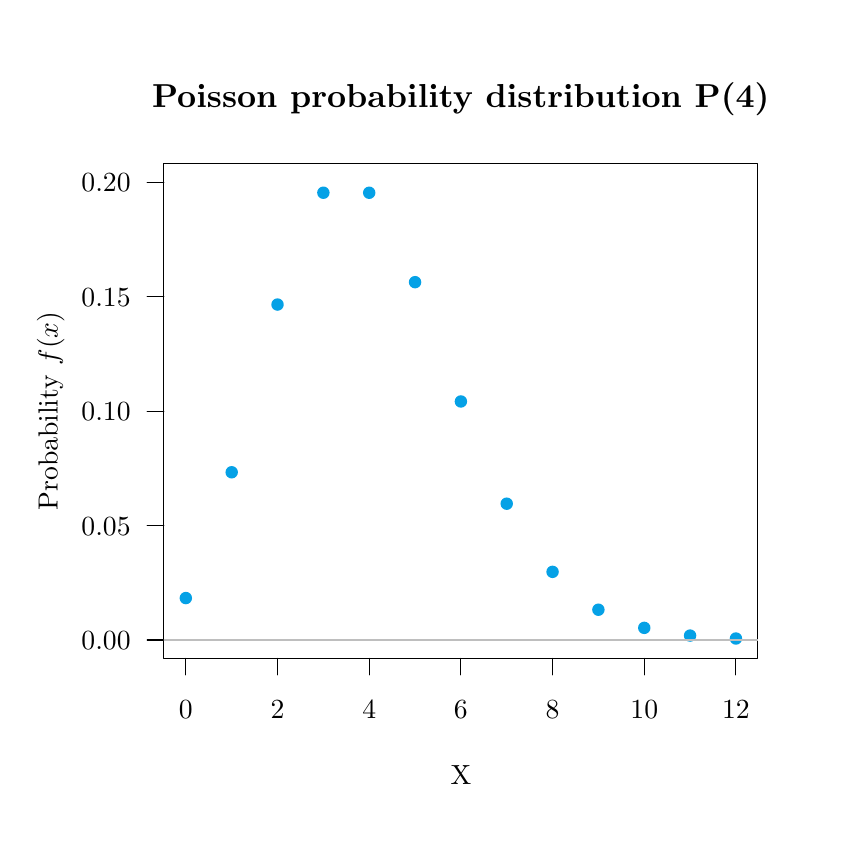
\begin{tikzpicture}[x=1pt,y=1pt]
\definecolor{fillColor}{RGB}{255,255,255}
\path[use as bounding box,fill=fillColor,fill opacity=0.00] (0,0) rectangle (289.08,289.08);
\begin{scope}
\path[clip] ( 49.20, 61.20) rectangle (263.88,239.88);
\definecolor{fillColor}{RGB}{5,161,230}

\path[fill=fillColor] ( 57.15, 82.97) circle (  2.25);

\path[fill=fillColor] ( 73.72,128.42) circle (  2.25);

\path[fill=fillColor] ( 90.28,189.03) circle (  2.25);

\path[fill=fillColor] (106.85,229.43) circle (  2.25);

\path[fill=fillColor] (123.41,229.43) circle (  2.25);

\path[fill=fillColor] (139.98,197.11) circle (  2.25);

\path[fill=fillColor] (156.54,154.01) circle (  2.25);

\path[fill=fillColor] (173.10,117.07) circle (  2.25);

\path[fill=fillColor] (189.67, 92.44) circle (  2.25);

\path[fill=fillColor] (206.23, 78.76) circle (  2.25);

\path[fill=fillColor] (222.80, 72.20) circle (  2.25);

\path[fill=fillColor] (239.36, 69.41) circle (  2.25);

\path[fill=fillColor] (255.93, 68.35) circle (  2.25);
\end{scope}
\begin{scope}
\path[clip] (  0.00,  0.00) rectangle (289.08,289.08);
\definecolor{drawColor}{RGB}{0,0,0}

\path[draw=drawColor,line width= 0.4pt,line join=round,line cap=round] ( 57.15, 61.20) -- (255.93, 61.20);

\path[draw=drawColor,line width= 0.4pt,line join=round,line cap=round] ( 57.15, 61.20) -- ( 57.15, 55.20);

\path[draw=drawColor,line width= 0.4pt,line join=round,line cap=round] ( 90.28, 61.20) -- ( 90.28, 55.20);

\path[draw=drawColor,line width= 0.4pt,line join=round,line cap=round] (123.41, 61.20) -- (123.41, 55.20);

\path[draw=drawColor,line width= 0.4pt,line join=round,line cap=round] (156.54, 61.20) -- (156.54, 55.20);

\path[draw=drawColor,line width= 0.4pt,line join=round,line cap=round] (189.67, 61.20) -- (189.67, 55.20);

\path[draw=drawColor,line width= 0.4pt,line join=round,line cap=round] (222.80, 61.20) -- (222.80, 55.20);

\path[draw=drawColor,line width= 0.4pt,line join=round,line cap=round] (255.93, 61.20) -- (255.93, 55.20);

\node[text=drawColor,anchor=base,inner sep=0pt, outer sep=0pt, scale=  1.00] at ( 57.15, 39.60) {0};

\node[text=drawColor,anchor=base,inner sep=0pt, outer sep=0pt, scale=  1.00] at ( 90.28, 39.60) {2};

\node[text=drawColor,anchor=base,inner sep=0pt, outer sep=0pt, scale=  1.00] at (123.41, 39.60) {4};

\node[text=drawColor,anchor=base,inner sep=0pt, outer sep=0pt, scale=  1.00] at (156.54, 39.60) {6};

\node[text=drawColor,anchor=base,inner sep=0pt, outer sep=0pt, scale=  1.00] at (189.67, 39.60) {8};

\node[text=drawColor,anchor=base,inner sep=0pt, outer sep=0pt, scale=  1.00] at (222.80, 39.60) {10};

\node[text=drawColor,anchor=base,inner sep=0pt, outer sep=0pt, scale=  1.00] at (255.93, 39.60) {12};

\path[draw=drawColor,line width= 0.4pt,line join=round,line cap=round] ( 49.20, 67.82) -- ( 49.20,233.26);

\path[draw=drawColor,line width= 0.4pt,line join=round,line cap=round] ( 49.20, 67.82) -- ( 43.20, 67.82);

\path[draw=drawColor,line width= 0.4pt,line join=round,line cap=round] ( 49.20,109.18) -- ( 43.20,109.18);

\path[draw=drawColor,line width= 0.4pt,line join=round,line cap=round] ( 49.20,150.54) -- ( 43.20,150.54);

\path[draw=drawColor,line width= 0.4pt,line join=round,line cap=round] ( 49.20,191.90) -- ( 43.20,191.90);

\path[draw=drawColor,line width= 0.4pt,line join=round,line cap=round] ( 49.20,233.26) -- ( 43.20,233.26);

\node[text=drawColor,anchor=base east,inner sep=0pt, outer sep=0pt, scale=  1.00] at ( 37.20, 64.37) {0.00};

\node[text=drawColor,anchor=base east,inner sep=0pt, outer sep=0pt, scale=  1.00] at ( 37.20,105.73) {0.05};

\node[text=drawColor,anchor=base east,inner sep=0pt, outer sep=0pt, scale=  1.00] at ( 37.20,147.10) {0.10};

\node[text=drawColor,anchor=base east,inner sep=0pt, outer sep=0pt, scale=  1.00] at ( 37.20,188.46) {0.15};

\node[text=drawColor,anchor=base east,inner sep=0pt, outer sep=0pt, scale=  1.00] at ( 37.20,229.82) {0.20};

\path[draw=drawColor,line width= 0.4pt,line join=round,line cap=round] ( 49.20, 61.20) --
	(263.88, 61.20) --
	(263.88,239.88) --
	( 49.20,239.88) --
	( 49.20, 61.20);
\end{scope}
\begin{scope}
\path[clip] (  0.00,  0.00) rectangle (289.08,289.08);
\definecolor{drawColor}{RGB}{0,0,0}

\node[text=drawColor,anchor=base,inner sep=0pt, outer sep=0pt, scale=  1.20] at (156.54,260.29) {\bfseries Poisson probability distribution P(4)};

\node[text=drawColor,anchor=base,inner sep=0pt, outer sep=0pt, scale=  1.00] at (156.54, 15.60) {X};

\node[text=drawColor,rotate= 90.00,anchor=base,inner sep=0pt, outer sep=0pt, scale=  1.00] at ( 10.80,150.54) {Probability $f(x)$};
\end{scope}
\begin{scope}
\path[clip] ( 49.20, 61.20) rectangle (263.88,239.88);
\definecolor{drawColor}{RGB}{190,190,190}

\path[draw=drawColor,line width= 0.4pt,line join=round,line cap=round] ( 49.20, 67.82) -- (263.88, 67.82);
\end{scope}
\end{tikzpicture}
}}
\mode<presentation>{\resizebox{0.55\textwidth}{!}{% Created by tikzDevice version 0.10.1 on 2016-04-19 09:52:58
% !TEX encoding = UTF-8 Unicode
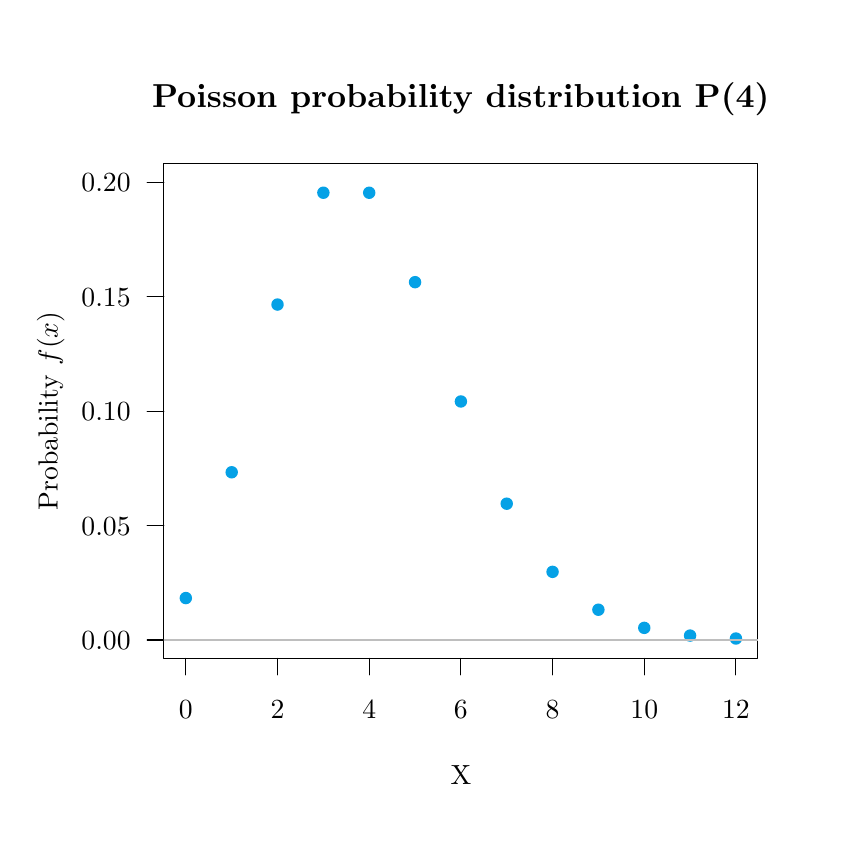
\begin{tikzpicture}[x=1pt,y=1pt]
\definecolor{fillColor}{RGB}{255,255,255}
\path[use as bounding box,fill=fillColor,fill opacity=0.00] (0,0) rectangle (289.08,289.08);
\begin{scope}
\path[clip] ( 49.20, 61.20) rectangle (263.88,239.88);
\definecolor{fillColor}{RGB}{5,161,230}

\path[fill=fillColor] ( 57.15, 82.97) circle (  2.25);

\path[fill=fillColor] ( 73.72,128.42) circle (  2.25);

\path[fill=fillColor] ( 90.28,189.03) circle (  2.25);

\path[fill=fillColor] (106.85,229.43) circle (  2.25);

\path[fill=fillColor] (123.41,229.43) circle (  2.25);

\path[fill=fillColor] (139.98,197.11) circle (  2.25);

\path[fill=fillColor] (156.54,154.01) circle (  2.25);

\path[fill=fillColor] (173.10,117.07) circle (  2.25);

\path[fill=fillColor] (189.67, 92.44) circle (  2.25);

\path[fill=fillColor] (206.23, 78.76) circle (  2.25);

\path[fill=fillColor] (222.80, 72.20) circle (  2.25);

\path[fill=fillColor] (239.36, 69.41) circle (  2.25);

\path[fill=fillColor] (255.93, 68.35) circle (  2.25);
\end{scope}
\begin{scope}
\path[clip] (  0.00,  0.00) rectangle (289.08,289.08);
\definecolor{drawColor}{RGB}{0,0,0}

\path[draw=drawColor,line width= 0.4pt,line join=round,line cap=round] ( 57.15, 61.20) -- (255.93, 61.20);

\path[draw=drawColor,line width= 0.4pt,line join=round,line cap=round] ( 57.15, 61.20) -- ( 57.15, 55.20);

\path[draw=drawColor,line width= 0.4pt,line join=round,line cap=round] ( 90.28, 61.20) -- ( 90.28, 55.20);

\path[draw=drawColor,line width= 0.4pt,line join=round,line cap=round] (123.41, 61.20) -- (123.41, 55.20);

\path[draw=drawColor,line width= 0.4pt,line join=round,line cap=round] (156.54, 61.20) -- (156.54, 55.20);

\path[draw=drawColor,line width= 0.4pt,line join=round,line cap=round] (189.67, 61.20) -- (189.67, 55.20);

\path[draw=drawColor,line width= 0.4pt,line join=round,line cap=round] (222.80, 61.20) -- (222.80, 55.20);

\path[draw=drawColor,line width= 0.4pt,line join=round,line cap=round] (255.93, 61.20) -- (255.93, 55.20);

\node[text=drawColor,anchor=base,inner sep=0pt, outer sep=0pt, scale=  1.00] at ( 57.15, 39.60) {0};

\node[text=drawColor,anchor=base,inner sep=0pt, outer sep=0pt, scale=  1.00] at ( 90.28, 39.60) {2};

\node[text=drawColor,anchor=base,inner sep=0pt, outer sep=0pt, scale=  1.00] at (123.41, 39.60) {4};

\node[text=drawColor,anchor=base,inner sep=0pt, outer sep=0pt, scale=  1.00] at (156.54, 39.60) {6};

\node[text=drawColor,anchor=base,inner sep=0pt, outer sep=0pt, scale=  1.00] at (189.67, 39.60) {8};

\node[text=drawColor,anchor=base,inner sep=0pt, outer sep=0pt, scale=  1.00] at (222.80, 39.60) {10};

\node[text=drawColor,anchor=base,inner sep=0pt, outer sep=0pt, scale=  1.00] at (255.93, 39.60) {12};

\path[draw=drawColor,line width= 0.4pt,line join=round,line cap=round] ( 49.20, 67.82) -- ( 49.20,233.26);

\path[draw=drawColor,line width= 0.4pt,line join=round,line cap=round] ( 49.20, 67.82) -- ( 43.20, 67.82);

\path[draw=drawColor,line width= 0.4pt,line join=round,line cap=round] ( 49.20,109.18) -- ( 43.20,109.18);

\path[draw=drawColor,line width= 0.4pt,line join=round,line cap=round] ( 49.20,150.54) -- ( 43.20,150.54);

\path[draw=drawColor,line width= 0.4pt,line join=round,line cap=round] ( 49.20,191.90) -- ( 43.20,191.90);

\path[draw=drawColor,line width= 0.4pt,line join=round,line cap=round] ( 49.20,233.26) -- ( 43.20,233.26);

\node[text=drawColor,anchor=base east,inner sep=0pt, outer sep=0pt, scale=  1.00] at ( 37.20, 64.37) {0.00};

\node[text=drawColor,anchor=base east,inner sep=0pt, outer sep=0pt, scale=  1.00] at ( 37.20,105.73) {0.05};

\node[text=drawColor,anchor=base east,inner sep=0pt, outer sep=0pt, scale=  1.00] at ( 37.20,147.10) {0.10};

\node[text=drawColor,anchor=base east,inner sep=0pt, outer sep=0pt, scale=  1.00] at ( 37.20,188.46) {0.15};

\node[text=drawColor,anchor=base east,inner sep=0pt, outer sep=0pt, scale=  1.00] at ( 37.20,229.82) {0.20};

\path[draw=drawColor,line width= 0.4pt,line join=round,line cap=round] ( 49.20, 61.20) --
	(263.88, 61.20) --
	(263.88,239.88) --
	( 49.20,239.88) --
	( 49.20, 61.20);
\end{scope}
\begin{scope}
\path[clip] (  0.00,  0.00) rectangle (289.08,289.08);
\definecolor{drawColor}{RGB}{0,0,0}

\node[text=drawColor,anchor=base,inner sep=0pt, outer sep=0pt, scale=  1.20] at (156.54,260.29) {\bfseries Poisson probability distribution P(4)};

\node[text=drawColor,anchor=base,inner sep=0pt, outer sep=0pt, scale=  1.00] at (156.54, 15.60) {X};

\node[text=drawColor,rotate= 90.00,anchor=base,inner sep=0pt, outer sep=0pt, scale=  1.00] at ( 10.80,150.54) {Probability $f(x)$};
\end{scope}
\begin{scope}
\path[clip] ( 49.20, 61.20) rectangle (263.88,239.88);
\definecolor{drawColor}{RGB}{190,190,190}

\path[draw=drawColor,line width= 0.4pt,line join=round,line cap=round] ( 49.20, 67.82) -- (263.88, 67.82);
\end{scope}
\end{tikzpicture}
}}
\end{center}
\end{frame}


%---------------------------------------------------------------------slide----
\begin{frame}
\frametitle{Poisson distribution model $P(\lambda)$}
\framesubtitle{Example of number of births in a city}
If $X\sim P(4)$ is the random variable that measures the number of births in the city, then
\begin{itemize}
\item The probability that there are 5 births in a day is
\[
f(5) = e^{-4}\frac{4^5}{5!} = 0.1563.
\]
\item The probability that there are less than 2 births in a day is
\[
F(1) = f(0)+f(1) = e^{-4}\frac{4^0}{0!} + e^{-4}\frac{4^1}{1!} = 5e^{-4} = 0.0916.
\]
\item The probability that there are more than 1 birth a day is 
\[
P(X>1) = 1-P(X\leq 1) = 1-F(1) = 1-0.0916 = 0.9084.
\]
\end{itemize}
\end{frame}


%---------------------------------------------------------------------slide----
\begin{frame}
\frametitle{Approximation of Binomial by Poisson distribution}
\framesubtitle{Law of rare events}
The Poisson distribution can be obtained from the Binomial distribution when the number of trials repetition tends to
infinite and the probability of Success tends to zero. 

\begin{theorem}[Law or rare events]
The Binomial distribution $X\sim B(n,p)$ tends to the Poisson distribution $P(\lambda)$, with $\lambda=n\cdot p$, when
$n$ tends to infinite and $p$ tends to zero, that is,
\[
\lim_{n\rightarrow \infty, p\rightarrow 0}\binom{n}{x}p^x(1-p)^{n-x} = e^{-\lambda}\frac{\lambda^x}{x!}.
\]
\end{theorem}

In practice, this approximation can be used for $n\geq 30$ and $p\leq 0.1$.
\end{frame}


%---------------------------------------------------------------------slide----
\begin{frame}
\frametitle{Approximation of Binomial by Poisson distribution}
\begin{center}
\tikzsetnextfilename{discrete_random_variables/law_rare_events}
\mode<article>{\resizebox{0.6\textwidth}{!}{% Created by tikzDevice version 0.10.1 on 2016-04-19 18:05:50
% !TEX encoding = UTF-8 Unicode
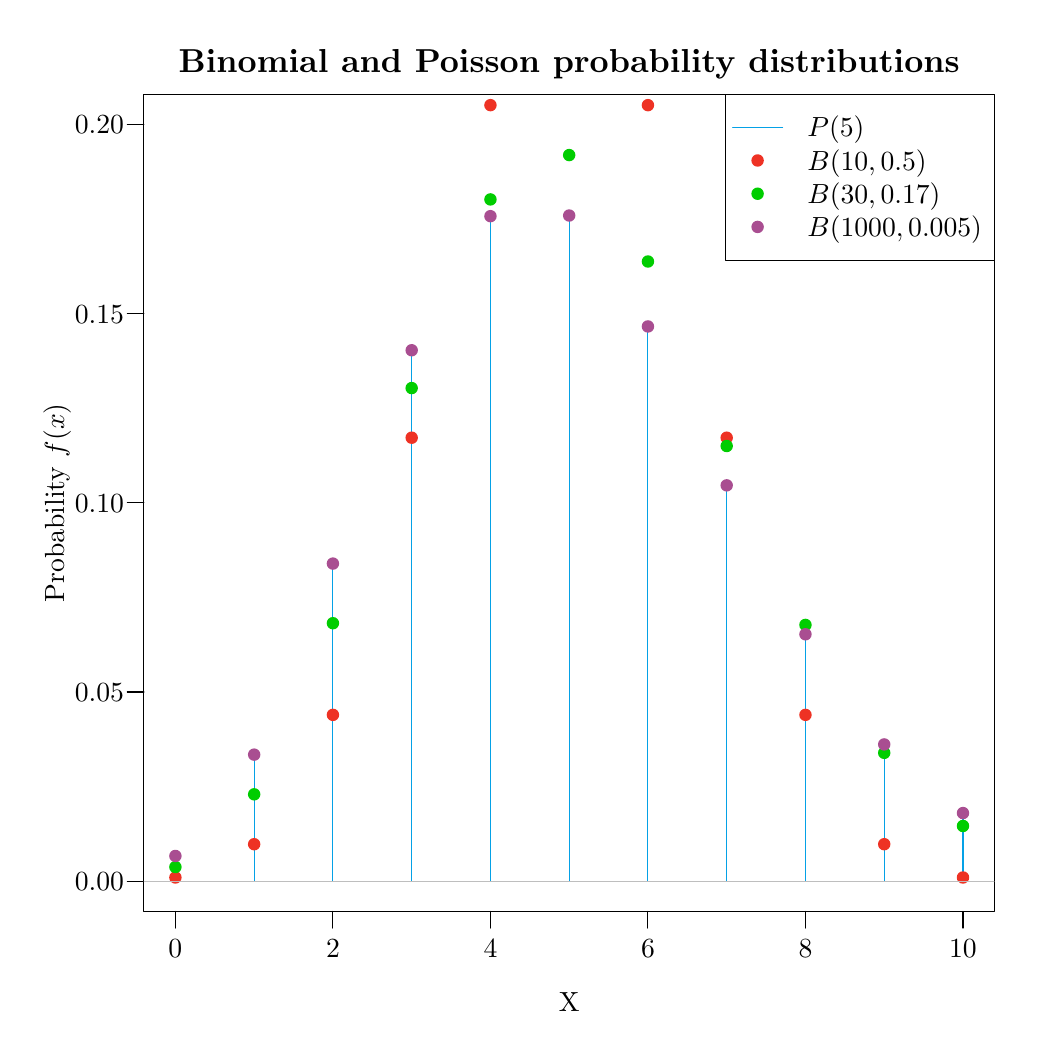
\begin{tikzpicture}[x=1pt,y=1pt]
\definecolor{fillColor}{RGB}{255,255,255}
\path[use as bounding box,fill=fillColor,fill opacity=0.00] (0,0) rectangle (361.35,361.35);
\begin{scope}
\path[clip] ( 42.00, 42.00) rectangle (349.35,337.35);
\definecolor{drawColor}{RGB}{5,161,230}

\path[draw=drawColor,line width= 0.4pt,line join=round,line cap=round] ( 53.38, 52.94) -- ( 53.38, 62.15);

\path[draw=drawColor,line width= 0.4pt,line join=round,line cap=round] ( 81.84, 52.94) -- ( 81.84, 99.00);

\path[draw=drawColor,line width= 0.4pt,line join=round,line cap=round] (110.30, 52.94) -- (110.30,168.10);

\path[draw=drawColor,line width= 0.4pt,line join=round,line cap=round] (138.76, 52.94) -- (138.76,244.88);

\path[draw=drawColor,line width= 0.4pt,line join=round,line cap=round] (167.22, 52.94) -- (167.22,292.87);

\path[draw=drawColor,line width= 0.4pt,line join=round,line cap=round] (195.67, 52.94) -- (195.67,292.87);

\path[draw=drawColor,line width= 0.4pt,line join=round,line cap=round] (224.13, 52.94) -- (224.13,252.88);

\path[draw=drawColor,line width= 0.4pt,line join=round,line cap=round] (252.59, 52.94) -- (252.59,195.75);

\path[draw=drawColor,line width= 0.4pt,line join=round,line cap=round] (281.05, 52.94) -- (281.05,142.20);

\path[draw=drawColor,line width= 0.4pt,line join=round,line cap=round] (309.51, 52.94) -- (309.51,102.53);

\path[draw=drawColor,line width= 0.4pt,line join=round,line cap=round] (337.97, 52.94) -- (337.97, 77.73);
\end{scope}
\begin{scope}
\path[clip] (  0.00,  0.00) rectangle (361.35,361.35);
\definecolor{drawColor}{RGB}{0,0,0}

\path[draw=drawColor,line width= 0.4pt,line join=round,line cap=round] ( 53.38, 42.00) -- (337.97, 42.00);

\path[draw=drawColor,line width= 0.4pt,line join=round,line cap=round] ( 53.38, 42.00) -- ( 53.38, 36.00);

\path[draw=drawColor,line width= 0.4pt,line join=round,line cap=round] (110.30, 42.00) -- (110.30, 36.00);

\path[draw=drawColor,line width= 0.4pt,line join=round,line cap=round] (167.22, 42.00) -- (167.22, 36.00);

\path[draw=drawColor,line width= 0.4pt,line join=round,line cap=round] (224.13, 42.00) -- (224.13, 36.00);

\path[draw=drawColor,line width= 0.4pt,line join=round,line cap=round] (281.05, 42.00) -- (281.05, 36.00);

\path[draw=drawColor,line width= 0.4pt,line join=round,line cap=round] (337.97, 42.00) -- (337.97, 36.00);

\node[text=drawColor,anchor=base,inner sep=0pt, outer sep=0pt, scale=  1.00] at ( 53.38, 25.20) {0};

\node[text=drawColor,anchor=base,inner sep=0pt, outer sep=0pt, scale=  1.00] at (110.30, 25.20) {2};

\node[text=drawColor,anchor=base,inner sep=0pt, outer sep=0pt, scale=  1.00] at (167.22, 25.20) {4};

\node[text=drawColor,anchor=base,inner sep=0pt, outer sep=0pt, scale=  1.00] at (224.13, 25.20) {6};

\node[text=drawColor,anchor=base,inner sep=0pt, outer sep=0pt, scale=  1.00] at (281.05, 25.20) {8};

\node[text=drawColor,anchor=base,inner sep=0pt, outer sep=0pt, scale=  1.00] at (337.97, 25.20) {10};

\path[draw=drawColor,line width= 0.4pt,line join=round,line cap=round] ( 42.00, 52.94) -- ( 42.00,326.41);

\path[draw=drawColor,line width= 0.4pt,line join=round,line cap=round] ( 42.00, 52.94) -- ( 36.00, 52.94);

\path[draw=drawColor,line width= 0.4pt,line join=round,line cap=round] ( 42.00,121.31) -- ( 36.00,121.31);

\path[draw=drawColor,line width= 0.4pt,line join=round,line cap=round] ( 42.00,189.67) -- ( 36.00,189.67);

\path[draw=drawColor,line width= 0.4pt,line join=round,line cap=round] ( 42.00,258.04) -- ( 36.00,258.04);

\path[draw=drawColor,line width= 0.4pt,line join=round,line cap=round] ( 42.00,326.41) -- ( 36.00,326.41);

\node[text=drawColor,anchor=base east,inner sep=0pt, outer sep=0pt, scale=  1.00] at ( 34.80, 49.49) {0.00};

\node[text=drawColor,anchor=base east,inner sep=0pt, outer sep=0pt, scale=  1.00] at ( 34.80,117.86) {0.05};

\node[text=drawColor,anchor=base east,inner sep=0pt, outer sep=0pt, scale=  1.00] at ( 34.80,186.23) {0.10};

\node[text=drawColor,anchor=base east,inner sep=0pt, outer sep=0pt, scale=  1.00] at ( 34.80,254.60) {0.15};

\node[text=drawColor,anchor=base east,inner sep=0pt, outer sep=0pt, scale=  1.00] at ( 34.80,322.97) {0.20};

\path[draw=drawColor,line width= 0.4pt,line join=round,line cap=round] ( 42.00, 42.00) --
	(349.35, 42.00) --
	(349.35,337.35) --
	( 42.00,337.35) --
	( 42.00, 42.00);
\end{scope}
\begin{scope}
\path[clip] (  0.00,  0.00) rectangle (361.35,361.35);
\definecolor{drawColor}{RGB}{0,0,0}

\node[text=drawColor,anchor=base,inner sep=0pt, outer sep=0pt, scale=  1.20] at (195.67,345.16) {\bfseries Binomial and Poisson probability distributions};

\node[text=drawColor,anchor=base,inner sep=0pt, outer sep=0pt, scale=  1.00] at (195.67,  6.00) {X};

\node[text=drawColor,rotate= 90.00,anchor=base,inner sep=0pt, outer sep=0pt, scale=  1.00] at ( 13.20,189.67) {Probability $f(x)$};
\end{scope}
\begin{scope}
\path[clip] ( 42.00, 42.00) rectangle (349.35,337.35);
\definecolor{fillColor}{RGB}{238,50,36}

\path[fill=fillColor] ( 53.38, 54.27) circle (  2.25);

\path[fill=fillColor] ( 81.84, 66.29) circle (  2.25);

\path[fill=fillColor] (110.30,113.03) circle (  2.25);

\path[fill=fillColor] (138.76,213.18) circle (  2.25);

\path[fill=fillColor] (167.22,333.35) circle (  2.25);

\path[fill=fillColor] (224.13,333.35) circle (  2.25);

\path[fill=fillColor] (252.59,213.18) circle (  2.25);

\path[fill=fillColor] (281.05,113.03) circle (  2.25);

\path[fill=fillColor] (309.51, 66.29) circle (  2.25);

\path[fill=fillColor] (337.97, 54.27) circle (  2.25);
\definecolor{fillColor}{RGB}{0,205,0}

\path[fill=fillColor] ( 53.38, 58.05) circle (  2.25);

\path[fill=fillColor] ( 81.84, 84.32) circle (  2.25);

\path[fill=fillColor] (110.30,146.15) circle (  2.25);

\path[fill=fillColor] (138.76,231.12) circle (  2.25);

\path[fill=fillColor] (167.22,299.28) circle (  2.25);

\path[fill=fillColor] (195.67,315.31) circle (  2.25);

\path[fill=fillColor] (224.13,276.85) circle (  2.25);

\path[fill=fillColor] (252.59,210.18) circle (  2.25);

\path[fill=fillColor] (281.05,145.53) circle (  2.25);

\path[fill=fillColor] (309.51, 99.30) circle (  2.25);

\path[fill=fillColor] (337.97, 72.88) circle (  2.25);
\definecolor{fillColor}{RGB}{169,78,145}

\path[fill=fillColor] ( 53.38, 62.04) circle (  2.25);

\path[fill=fillColor] ( 81.84, 98.66) circle (  2.25);

\path[fill=fillColor] (110.30,167.70) circle (  2.25);

\path[fill=fillColor] (138.76,244.78) circle (  2.25);

\path[fill=fillColor] (167.22,293.23) circle (  2.25);

\path[fill=fillColor] (195.67,293.47) circle (  2.25);

\path[fill=fillColor] (224.13,253.38) circle (  2.25);

\path[fill=fillColor] (252.59,195.97) circle (  2.25);

\path[fill=fillColor] (281.05,142.15) circle (  2.25);

\path[fill=fillColor] (309.51,102.35) circle (  2.25);

\path[fill=fillColor] (337.97, 77.55) circle (  2.25);
\definecolor{drawColor}{RGB}{190,190,190}

\path[draw=drawColor,line width= 0.4pt,line join=round,line cap=round] ( 42.00, 52.94) -- (349.35, 52.94);
\definecolor{drawColor}{RGB}{0,0,0}

\path[draw=drawColor,line width= 0.4pt,line join=round,line cap=round] (252.06,337.35) rectangle (349.35,277.35);
\definecolor{drawColor}{RGB}{5,161,230}

\path[draw=drawColor,line width= 0.4pt,line join=round,line cap=round] (254.76,325.35) -- (272.76,325.35);
\definecolor{fillColor}{RGB}{238,50,36}

\path[fill=fillColor] (263.76,313.35) circle (  2.25);
\definecolor{fillColor}{RGB}{0,205,0}

\path[fill=fillColor] (263.76,301.35) circle (  2.25);
\definecolor{fillColor}{RGB}{169,78,145}

\path[fill=fillColor] (263.76,289.35) circle (  2.25);
\definecolor{drawColor}{RGB}{0,0,0}

\node[text=drawColor,anchor=base west,inner sep=0pt, outer sep=0pt, scale=  1.00] at (281.76,321.91) {$P(5)$};

\node[text=drawColor,anchor=base west,inner sep=0pt, outer sep=0pt, scale=  1.00] at (281.76,309.91) {$B(10,0.5)$};

\node[text=drawColor,anchor=base west,inner sep=0pt, outer sep=0pt, scale=  1.00] at (281.76,297.91) {$B(30,0.17)$};

\node[text=drawColor,anchor=base west,inner sep=0pt, outer sep=0pt, scale=  1.00] at (281.76,285.91) {$B(1000,0.005)$};
\end{scope}
\end{tikzpicture}
}}
\mode<presentation>{\resizebox{0.65\textwidth}{!}{% Created by tikzDevice version 0.10.1 on 2016-04-19 18:05:50
% !TEX encoding = UTF-8 Unicode
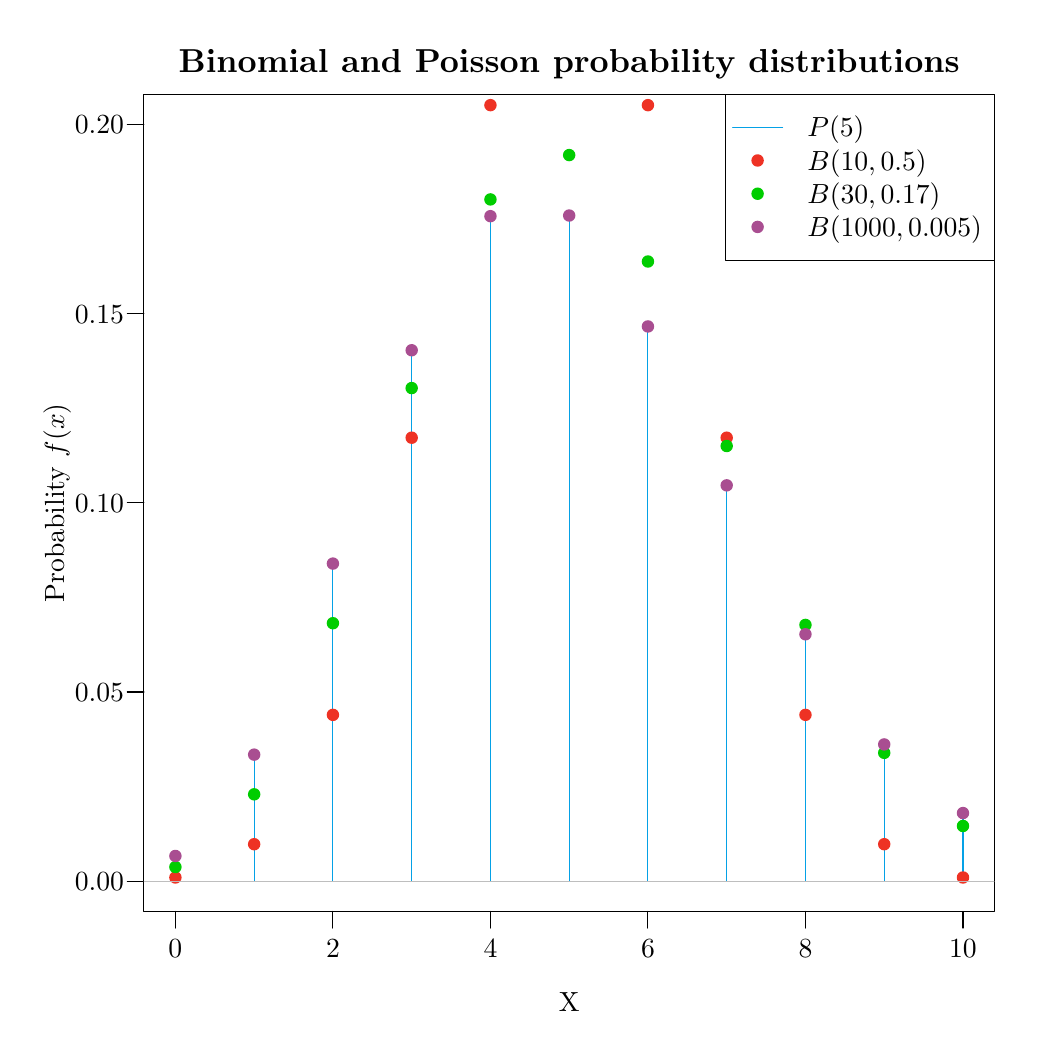
\begin{tikzpicture}[x=1pt,y=1pt]
\definecolor{fillColor}{RGB}{255,255,255}
\path[use as bounding box,fill=fillColor,fill opacity=0.00] (0,0) rectangle (361.35,361.35);
\begin{scope}
\path[clip] ( 42.00, 42.00) rectangle (349.35,337.35);
\definecolor{drawColor}{RGB}{5,161,230}

\path[draw=drawColor,line width= 0.4pt,line join=round,line cap=round] ( 53.38, 52.94) -- ( 53.38, 62.15);

\path[draw=drawColor,line width= 0.4pt,line join=round,line cap=round] ( 81.84, 52.94) -- ( 81.84, 99.00);

\path[draw=drawColor,line width= 0.4pt,line join=round,line cap=round] (110.30, 52.94) -- (110.30,168.10);

\path[draw=drawColor,line width= 0.4pt,line join=round,line cap=round] (138.76, 52.94) -- (138.76,244.88);

\path[draw=drawColor,line width= 0.4pt,line join=round,line cap=round] (167.22, 52.94) -- (167.22,292.87);

\path[draw=drawColor,line width= 0.4pt,line join=round,line cap=round] (195.67, 52.94) -- (195.67,292.87);

\path[draw=drawColor,line width= 0.4pt,line join=round,line cap=round] (224.13, 52.94) -- (224.13,252.88);

\path[draw=drawColor,line width= 0.4pt,line join=round,line cap=round] (252.59, 52.94) -- (252.59,195.75);

\path[draw=drawColor,line width= 0.4pt,line join=round,line cap=round] (281.05, 52.94) -- (281.05,142.20);

\path[draw=drawColor,line width= 0.4pt,line join=round,line cap=round] (309.51, 52.94) -- (309.51,102.53);

\path[draw=drawColor,line width= 0.4pt,line join=round,line cap=round] (337.97, 52.94) -- (337.97, 77.73);
\end{scope}
\begin{scope}
\path[clip] (  0.00,  0.00) rectangle (361.35,361.35);
\definecolor{drawColor}{RGB}{0,0,0}

\path[draw=drawColor,line width= 0.4pt,line join=round,line cap=round] ( 53.38, 42.00) -- (337.97, 42.00);

\path[draw=drawColor,line width= 0.4pt,line join=round,line cap=round] ( 53.38, 42.00) -- ( 53.38, 36.00);

\path[draw=drawColor,line width= 0.4pt,line join=round,line cap=round] (110.30, 42.00) -- (110.30, 36.00);

\path[draw=drawColor,line width= 0.4pt,line join=round,line cap=round] (167.22, 42.00) -- (167.22, 36.00);

\path[draw=drawColor,line width= 0.4pt,line join=round,line cap=round] (224.13, 42.00) -- (224.13, 36.00);

\path[draw=drawColor,line width= 0.4pt,line join=round,line cap=round] (281.05, 42.00) -- (281.05, 36.00);

\path[draw=drawColor,line width= 0.4pt,line join=round,line cap=round] (337.97, 42.00) -- (337.97, 36.00);

\node[text=drawColor,anchor=base,inner sep=0pt, outer sep=0pt, scale=  1.00] at ( 53.38, 25.20) {0};

\node[text=drawColor,anchor=base,inner sep=0pt, outer sep=0pt, scale=  1.00] at (110.30, 25.20) {2};

\node[text=drawColor,anchor=base,inner sep=0pt, outer sep=0pt, scale=  1.00] at (167.22, 25.20) {4};

\node[text=drawColor,anchor=base,inner sep=0pt, outer sep=0pt, scale=  1.00] at (224.13, 25.20) {6};

\node[text=drawColor,anchor=base,inner sep=0pt, outer sep=0pt, scale=  1.00] at (281.05, 25.20) {8};

\node[text=drawColor,anchor=base,inner sep=0pt, outer sep=0pt, scale=  1.00] at (337.97, 25.20) {10};

\path[draw=drawColor,line width= 0.4pt,line join=round,line cap=round] ( 42.00, 52.94) -- ( 42.00,326.41);

\path[draw=drawColor,line width= 0.4pt,line join=round,line cap=round] ( 42.00, 52.94) -- ( 36.00, 52.94);

\path[draw=drawColor,line width= 0.4pt,line join=round,line cap=round] ( 42.00,121.31) -- ( 36.00,121.31);

\path[draw=drawColor,line width= 0.4pt,line join=round,line cap=round] ( 42.00,189.67) -- ( 36.00,189.67);

\path[draw=drawColor,line width= 0.4pt,line join=round,line cap=round] ( 42.00,258.04) -- ( 36.00,258.04);

\path[draw=drawColor,line width= 0.4pt,line join=round,line cap=round] ( 42.00,326.41) -- ( 36.00,326.41);

\node[text=drawColor,anchor=base east,inner sep=0pt, outer sep=0pt, scale=  1.00] at ( 34.80, 49.49) {0.00};

\node[text=drawColor,anchor=base east,inner sep=0pt, outer sep=0pt, scale=  1.00] at ( 34.80,117.86) {0.05};

\node[text=drawColor,anchor=base east,inner sep=0pt, outer sep=0pt, scale=  1.00] at ( 34.80,186.23) {0.10};

\node[text=drawColor,anchor=base east,inner sep=0pt, outer sep=0pt, scale=  1.00] at ( 34.80,254.60) {0.15};

\node[text=drawColor,anchor=base east,inner sep=0pt, outer sep=0pt, scale=  1.00] at ( 34.80,322.97) {0.20};

\path[draw=drawColor,line width= 0.4pt,line join=round,line cap=round] ( 42.00, 42.00) --
	(349.35, 42.00) --
	(349.35,337.35) --
	( 42.00,337.35) --
	( 42.00, 42.00);
\end{scope}
\begin{scope}
\path[clip] (  0.00,  0.00) rectangle (361.35,361.35);
\definecolor{drawColor}{RGB}{0,0,0}

\node[text=drawColor,anchor=base,inner sep=0pt, outer sep=0pt, scale=  1.20] at (195.67,345.16) {\bfseries Binomial and Poisson probability distributions};

\node[text=drawColor,anchor=base,inner sep=0pt, outer sep=0pt, scale=  1.00] at (195.67,  6.00) {X};

\node[text=drawColor,rotate= 90.00,anchor=base,inner sep=0pt, outer sep=0pt, scale=  1.00] at ( 13.20,189.67) {Probability $f(x)$};
\end{scope}
\begin{scope}
\path[clip] ( 42.00, 42.00) rectangle (349.35,337.35);
\definecolor{fillColor}{RGB}{238,50,36}

\path[fill=fillColor] ( 53.38, 54.27) circle (  2.25);

\path[fill=fillColor] ( 81.84, 66.29) circle (  2.25);

\path[fill=fillColor] (110.30,113.03) circle (  2.25);

\path[fill=fillColor] (138.76,213.18) circle (  2.25);

\path[fill=fillColor] (167.22,333.35) circle (  2.25);

\path[fill=fillColor] (224.13,333.35) circle (  2.25);

\path[fill=fillColor] (252.59,213.18) circle (  2.25);

\path[fill=fillColor] (281.05,113.03) circle (  2.25);

\path[fill=fillColor] (309.51, 66.29) circle (  2.25);

\path[fill=fillColor] (337.97, 54.27) circle (  2.25);
\definecolor{fillColor}{RGB}{0,205,0}

\path[fill=fillColor] ( 53.38, 58.05) circle (  2.25);

\path[fill=fillColor] ( 81.84, 84.32) circle (  2.25);

\path[fill=fillColor] (110.30,146.15) circle (  2.25);

\path[fill=fillColor] (138.76,231.12) circle (  2.25);

\path[fill=fillColor] (167.22,299.28) circle (  2.25);

\path[fill=fillColor] (195.67,315.31) circle (  2.25);

\path[fill=fillColor] (224.13,276.85) circle (  2.25);

\path[fill=fillColor] (252.59,210.18) circle (  2.25);

\path[fill=fillColor] (281.05,145.53) circle (  2.25);

\path[fill=fillColor] (309.51, 99.30) circle (  2.25);

\path[fill=fillColor] (337.97, 72.88) circle (  2.25);
\definecolor{fillColor}{RGB}{169,78,145}

\path[fill=fillColor] ( 53.38, 62.04) circle (  2.25);

\path[fill=fillColor] ( 81.84, 98.66) circle (  2.25);

\path[fill=fillColor] (110.30,167.70) circle (  2.25);

\path[fill=fillColor] (138.76,244.78) circle (  2.25);

\path[fill=fillColor] (167.22,293.23) circle (  2.25);

\path[fill=fillColor] (195.67,293.47) circle (  2.25);

\path[fill=fillColor] (224.13,253.38) circle (  2.25);

\path[fill=fillColor] (252.59,195.97) circle (  2.25);

\path[fill=fillColor] (281.05,142.15) circle (  2.25);

\path[fill=fillColor] (309.51,102.35) circle (  2.25);

\path[fill=fillColor] (337.97, 77.55) circle (  2.25);
\definecolor{drawColor}{RGB}{190,190,190}

\path[draw=drawColor,line width= 0.4pt,line join=round,line cap=round] ( 42.00, 52.94) -- (349.35, 52.94);
\definecolor{drawColor}{RGB}{0,0,0}

\path[draw=drawColor,line width= 0.4pt,line join=round,line cap=round] (252.06,337.35) rectangle (349.35,277.35);
\definecolor{drawColor}{RGB}{5,161,230}

\path[draw=drawColor,line width= 0.4pt,line join=round,line cap=round] (254.76,325.35) -- (272.76,325.35);
\definecolor{fillColor}{RGB}{238,50,36}

\path[fill=fillColor] (263.76,313.35) circle (  2.25);
\definecolor{fillColor}{RGB}{0,205,0}

\path[fill=fillColor] (263.76,301.35) circle (  2.25);
\definecolor{fillColor}{RGB}{169,78,145}

\path[fill=fillColor] (263.76,289.35) circle (  2.25);
\definecolor{drawColor}{RGB}{0,0,0}

\node[text=drawColor,anchor=base west,inner sep=0pt, outer sep=0pt, scale=  1.00] at (281.76,321.91) {$P(5)$};

\node[text=drawColor,anchor=base west,inner sep=0pt, outer sep=0pt, scale=  1.00] at (281.76,309.91) {$B(10,0.5)$};

\node[text=drawColor,anchor=base west,inner sep=0pt, outer sep=0pt, scale=  1.00] at (281.76,297.91) {$B(30,0.17)$};

\node[text=drawColor,anchor=base west,inner sep=0pt, outer sep=0pt, scale=  1.00] at (281.76,285.91) {$B(1000,0.005)$};
\end{scope}
\end{tikzpicture}
}}
\end{center}
\end{frame}


%---------------------------------------------------------------------slide----
\begin{frame}
\frametitle{Approximation of Binomial by Poisson distribution}
\framesubtitle{Example}
A vaccine produce an adverse reaction in 4\% of cases.
If a sample of 50 persons are vaccinated, what is the probability of having more than 2 persons with an adverse
reaction?

The variable that measures the number of persons with an adverse reaction in the sample follows a Binomial distribution
model $X\sim B(50,0.04)$, but as $n=50>30$ and $p=0.04<0.1$, we can apply the law of rare events and use the
Poisson distribution model $P(50\cdot 0.04)=P(2)$ to do the calculations. 
\begin{align*}
P(X>2) &= 1-P(X\leq 2) = 1-f(0)-f(1)-f(2) =\\
&= 1-e^{-2}\frac{2^0}{0!}-e^{-2}\frac{2^1}{1!}-e^{-2}\frac{2^2}{2!} =\\
&= 1-5e^{-2} = 0.3233.
\end{align*}
\end{frame}

